\documentclass[a4paper,12pt,oneside]{book} % oneside permite que no haya una página en blanco despues de la portada
%\documentclass[a4paper,12pt,oneside,draft]{book} %PARA DEBUGEO \hbox

% #####################################################################
% ############################# PAQUETES ##############################
% #####################################################################

% ************************CODIFICACIÓN Y FUENTE************************
\usepackage[utf8]{inputenc}
\usepackage{mathptmx} % Defines Adobe Times Roman (or equivalent) as default text font
\pdfminorversion=7 % Por un warning por el logo en la portada

% ************************INTERNACIONALIZACIÓN************************
\usepackage[spanish,es-lcroman,es-nodecimaldot,es-tabla]{babel} % spanish, es-lcroman son para cambiar la numeración romana a mínuscula. (Por defecto, solo spanish esta en mayuscula), es-nodecimaldot es para usar "." como separador decimal

% ************************GEOMETRÍA Y MÁRGENES************************
\PassOptionsToPackage{showframe}{geometry} % Habilitar la opción de mostrar margenes en el paquete "geometry"
\usepackage[a4paper,left=2.54cm, right=2.54cm, top=2.54cm, bottom=2.54cm]{geometry} % Define los márgenes de la página

% *************************GRÁFICOS Y FIGURAS*************************
\usepackage{graphicx} % Permite incluir gráficos, \resizebox
\graphicspath{ {./img/} } % Ruta por defector para las imágenes

% ********************ENCABEZADOS Y PIES DE PÁGINA********************
\usepackage{fancyhdr} % Permite personalizar encabezados y pies de página
\setlength{\headheight}{14.5pt} % Para evitar un warning "Make it at least 14.49998pt"

% ******************************CAPTIONS******************************
%\usepackage[font=small]{caption} % Cambia el tamaño de las captions (figure y xltabular) a 10pt (ya que el documento esta definido en 12pt)
\usepackage{caption}
\captionsetup{
	format=plain,
	labelformat=simple,
	font=small,
	labelsep=colon,
	skip=6pt,
	justification=centering
}

% ****************************INTERLINEADO****************************
\usepackage{setspace} % Permite cambiar el interlineado, permite usar \doublespacing y tambien permite usar \begin{spacing} para que solo cierto texto tenga otro valor de interlineado

% *******************************TABLAS*******************************
\usepackage{xltabular} % Este paquete carga el paquete ltablex, pero mantiene el entorno tabularx actual tal como está. El nuevo entorno xltabular es una combinación de longtable y tabularx: definiciones de encabezado/pie de página, especificador de columna X y posibles saltos de página.
\usepackage{booktabs} % Para líneas horizontales profesionales: uso \toprule, \midrule, \bottomrule
\usepackage{array} % Para definir nuevos tipos de columna con alineación: uso \newcolumntype
\usepackage{tabularray,tblr-extras}
\UseTblrLibrary{caption}

% *******************************ÍNDICES*******************************
\usepackage[figurewithin=none]{caption} % Remueve el espacio entre items de distinto chapter en la Lista de figuras
\usepackage[tablewithin=none]{caption} % Remueve el espacio entre items de distinto chapter en la Lista de tablas
\usepackage{tocbibind} % Permite incluir el índice de tablas, figuras y la bibliografía al índice general
\usepackage{titletoc}% Personalización detallada de los contenidos, incluye \titlecontents

% ****************************SITUACIONALES****************************
\usepackage{lipsum} % Genera texto de relleno

% Now load showboxes:
%\usepackage{showboxes}
% Enable frame drawing around boxes:
%\ShowFrameBoxes

% ********************************OTROS********************************
\usepackage{titlesec} % Permite cambiar el tamaño, color, fuente de los títulos de chapter, section y subsection
\usepackage[hidelinks,hypertexnames=false]{hyperref} % Gestiona enlaces hipertexto, incluye (\url) y \phantomsection y % Para evitar un warning "destination with the same identifier..."
\usepackage[none]{hyphenat} % Para evitar que LaTeX corte las palabras al final de línea
\usepackage{xurl} % Permite cortar URLs largas automáticamente en saltos de línea sin errores de formato
%\usepackage{float} % Permite fijar la posición exacta de figuras/tablas con [H]
\usepackage{environ} % Permite crear el nuevo entorno my_xltabular

\usepackage{xcolor}
\definecolor{Cerulean}{rgb}{0,0.682,0.937}
\definecolor{Turbo}{rgb}{1,0.945,0.003}
\definecolor{GreenYellow}{rgb}{0.678,1,0.184}


\usepackage{colortbl}
\usepackage{multicol}
\usepackage{bigstrut}
\usepackage{float}




% #####################################################################
% ################### DEFINICIÓN DE NUEVOS COMANDOS ###################
% #####################################################################

% ------------------- COMANDO PARA IMPRIMIR EL MES ------------------
% Macro \mes: muestra el mes actual en español.
\newcommand{\mes}{%
	\ifcase\month\or Enero\or Febrero\or Marzo\or Abril\or Mayo\or Junio\or Julio\or Agosto\or Septiembre\or Octubre\or Noviembre\or Diciembre\fi}

% ------------------- CONFIGURAR FOOTERS Y HEADERS -------------------
% Se definen dos estilos, uno para el frontmatter con numeración en el centro-abajo; y mainmatterstyle, con numeración derecha-arriba
\fancypagestyle{frontmatterstyle}{ % Estilo para el frontmatter
	\fancyhf{} % Limpia el header and footer
	\fancyfoot[C]{\thepage} % En el centro del footer coloca la numeración
	\renewcommand{\headrulewidth}{0pt} % La línea se setea a grosor 0pt
}
\fancypagestyle{mainmatterstyle}{ % Estilo para el mainmatter
	\fancyhf{} % Limpia el header and footer
	\fancyhead[R]{\thepage} % En la esquina superior derecha del header coloca la numeración
	\renewcommand{\headrulewidth}{0pt} % La línea se setea a grosor 0pt
}

% ------------------ CONFIGURACIÓN DEL INTERLINEADO -------------------
\AtBeginEnvironment{figure}{\onehalfspacing} % Configura automáticamente interlineado simple en figuras
\AtBeginEnvironment{xltabular}{\onehalfspacing} % Configura automáticamente interlineado 1.5 en tablas xltabular
\AtBeginEnvironment{longtblr}{\onehalfspacing} % Configura automáticamente interlineado 1.5 en tablas xltabular

% -------- CONFIGURACIÓN DE FUENTES Y TAMAÑOS DE LOS TÍTULOS --------
% Personalización de \chapter
% - [display] : hace que el número y el título del capítulo se muestren en líneas separadas
% - Estilo del título de la sección
% - CAPÍTULO #N : Prefijo del título + Número del capítulo
% - 12pt : Espacio entre el prefijo y el título del capítulo.
% - {}: Código adicional para antes del título (vacío en este caso).
\titleformat{\chapter}[display]
{\singlespacing\normalsize\bfseries\centering}
{\MakeUppercase{\chaptertitlename} \thechapter}
{12pt}
{}

% Personalización de \section
% - Estilo del título de la sección: singlespacing, normalfont, normalsize, bfseries.
% - Prefijo del título, ej. "1.1": utiliza \thesection seguido de un punto.
% - 12pt: Espacio entre el prefijo y el título de la sección.
% - {}: Código adicional para antes del título (vacío en este caso).
\titleformat{\section}
{\singlespacing\normalsize\bfseries}
{\thesection.}
{6pt}
{}

% Personalización de \subsection
% - Estilo del título de la subsección: singlespacing, normalfont, normalsize, bfseries.
% - Prefijo del título, ej. "1.1.1": utiliza \thesubsection seguido de un punto.
% - 12pt: Espacio entre el prefijo y el título de la subsección.
% - {}: Código adicional para antes del título, si es necesario (vacío).
\titleformat{\subsection}
{\singlespacing\normalfont\normalsize\bfseries}
{\thesubsection.}
{12pt}
{}

% Reducción del espacio en blanco encima del \chapter
% - 0pt: Sin sangría a la izquierda
% - -24.5pt: Reduce el espacio vertical predeterminado antes del título.
% - 12pt: Espacio de 12pt después del título.
\titlespacing*{\chapter}{0pt}{-29.5pt}{12pt} 

% Reducción del espacio en blanco encima del \section
% - 0pt: Sin sangría a la izquierda
% - 0pt: Sin espacio vertical adicional antes del título.
% - 6pt: Espacio de 6pt después del título.
\titlespacing*{\section}{0pt}{0pt}{6pt}

% Reducción del espacio en blanco encima del \subsection
% - 0pt: Sin sangría a la izquierda.
% - 0pt: Sin espacio vertical adicional antes del título.
% - 6pt: Espacio de 6pt después del título.
\titlespacing*{\subsection}{0pt}{0pt}{6pt}

% ------------- CONFIGURACIÓN DE LA TABLA DE CONTENIDOS -------------
% Configuración de la entrada de capítulos en la tabla de contenido
% - Nivel de sección: chapter
% - 0pt: Sin sangría.
% - \vspace{6pt}\bfseries: Añade espacio vertical antes y aplica negrita al texto.
% - \MakeUppercase{\chaptername} \thecontentslabel: : Muestra el nombre del capítulo en mayúsculas y su número seguido de dos puntos.
% - {}: No se define un formato especial para entradas sin número.
% - \hfill\contentspage: Alinea el número de página a la derecha con puntos de relleno.
% - []: No hay código adicional después de la entrada.
\titlecontents{chapter}
[0pt]
{\vspace{6pt}\bfseries}
{\MakeUppercase{\chaptername} \thecontentslabel: }
{}
{\hfill\contentspage}
[]

% -------------- CONFIGURACIÓN DE UN NUEVO ENTORNO FIGURE --------------
% Crea una leyenda que incluye fuente: #1 es el título (usado en la lista y en la leyenda) y #2 la fuente.
\newcommand*{\captionsource}[2]{%
	\if\relax\detokenize{#2}\relax
	\caption[{#1}]{\centering #1.}%
	\else
	\caption[{#1}]{\centering #1.\\Fuente: Adaptado de #2}%
	\fi
}
% Define un comando para figuras con fuente y ancho parametrizado.
% #1: posición (e.g., h, t),
% #2: archivo de imagen,
% #3: título,
% #4: fuente (o cita)
% #5: ancho.
\newcommand{\sourcefigure}[5]{%
	\begin{figure}[#1]
		\centering
		\captionsetup{width=#5,belowskip=-10pt}
		\includegraphics[width=#5]{#2}
		\captionsource{#3}{#4}%
		\label{fig:#2}
	\end{figure}
}

% ----------------------- CONFIGURACIÓN DE longtblr ------------------------
\NewColumnType{Y}{Q[c,co=1]}
\DeclareTblrTemplate{contfoot-text}{normal}{Continua en la siguiente página...}
\SetTblrTemplate{contfoot-text}{normal}
\DeclareTblrTemplate{conthead-text}{normal}{\\(Continuación)}
\SetTblrTemplate{conthead-text}{normal}
\SetTblrInner[longtblr]{rowsep=0pt}

% Definición de la macro:
\newcommand{\bestTabla}[5][]{%
	\begin{longtblr}[%
		label   = {#1},%
		caption = {%
			#2%
			\if\relax\detokenize{#3}\relax
			.%  si #3 está vacío, sólo el punto
			\else
			. Fuente: Adaptado de #3% si #3 no está vacío
			\fi
		},%
		entry   = {#2}% siempre el primer argumento
		]{#4}%
		#5%
	\end{longtblr}%
}

% ------------------ EVITA EL WARNING DE UNDERFULL HBOXES ------------------
\hbadness=99999
\setlength\emergencystretch{10em} % Archivo de configuración de todo el documento

% ######################### INFORMACIÓN DEL DOCUMENTO #########################
\newcommand\documenttitle {[TÍTULO DE LA TESIS]}
\newcommand\documentauthor {[Colocar el nombre completo del autor según el registro de su DNI]}
\newcommand\documentauthorabbreviation {---N. Apellido---}
\newcommand\myadvisor{[Colocar el nombre completo del asesor según el registro de su DNI]}
\newcommand\mycoadvisor{-}
\newcommand\universityname {PONTIFICIA UNIVERSIDAD CATÓLICA DEL PERÚ}
\newcommand\universityfaculty {FACULTAD DE CIENCIAS E INGENIERÍA}
\newcommand\universityimage {logo_PUCP_antiguo.pdf}
\newcommand\universitylocation{Lima}
\newcommand\documentdate {\mes, \the\year}
%\def\documentsubtitle {1MTR01 Trabajo de Fin de Carrera 1}
\newcommand\documentsubtitle {1MTR02 Trabajo de Fin de Carrera 2}
%\def\documentsubtitle {Tesis para optener el título profesional de Ingeniero Mecatrónico}

\begin{document}
	
% RENOMBRANDO TÍTULOS DE LOS ÍNDICES
\renewcommand{\contentsname}{ÍNDICE DE CONTENIDO}
\renewcommand{\listtablename}{ÍNDICE DE TABLAS}
\renewcommand{\listfigurename}{ÍNDICE DE FIGURAS}
\renewcommand{\bibname}{BIBLIOGRAFÍA}

%==========================================================================

%%%%%% PORTADA

\begin{titlepage}
\centering
%%%% Cabecera
\large\textbf{\universityname}\\
\bigskip
\large\textbf{\universityfaculty}

%%%% Logo de la PUCP
\vskip 1.5cm
\includegraphics[scale=0.9]{\universityimage}

%%%% Titulo de la Tesis:
\vskip 1.5cm
\large\textbf{\documenttitle}

%%%% Datos del Tesista:
\vskip 1.5cm
\large\textbf{\documentsubtitle}
\vskip 2cm
\large\textbf{AUTOR:}\\
\large\documentauthor

%%%% Datos del Asesor:
\vskip 2.5cm
\large\textbf{ASESOR:}\\
\large\myadvisor \\
%\Large\textbf{CO-ASESOR:}\\
%\Large\mycoadvisor

%%%% Lugar y fecha:
\vskip 3.5cm
\large \universitylocation, \documentdate

\end{titlepage}

\clearpage

% Configuración de la numeración
\frontmatter % Inicia la numeración romana
\pagestyle{frontmatterstyle} % Numeración en el centro inferior
\pagenumbering{roman}

%%%%%% RESUMEN

\chapter*{RESUMEN}
\addcontentsline{toc}{chapter}{RESUMEN}

(El resumen debe presentar de forma breve, clara y concisa el contenido del trabajo, resaltando los objetivos, los métodos o procedimientos empleados, los resultados obtenidos y las conclusiones. El resumen no debe de tener más 300 palabras de extensión. Se escribe a espacio simple.)

\begin{itemize}
	\item La extensión debe ser de 200 a 300 palabras, sin exceder a una página.
	\item Escriba en tiempo verbal presente.
	\item El resumen debe contener información sobre:
	\begin{itemize}
		\item La justificación de la investigación
		\item Los objetivos o hipótesis
		\item La teoría o supuestos teóricos o metodológicos en la que se sustenta
		\item El método o procedimiento realizado (de ser necesario)
		\item Los resultados (de ser necesario)
		\item La conclusión principal
	\end{itemize}
\end{itemize}

\clearpage
\newpage

%%%%%% AGRADECIMIENTOS

\chapter*{AGRADECIMIENTOS}

\null\vspace{\stretch{1}}
    \begin{flushright}
            A mis padres por su incondicional apoyo durante todos estos años de carrera.
            
            A mi familia por la confianza depositada en mi.
            
            A mi asesor por ayudarme y orientarme en el desarrollo de esta tesis.
            
            A mis amigos por acompañarme durante toda esta experiencia.
    \end{flushright}
\vspace{\stretch{2}}\null

\clearpage
\newpage

%==========================================================================

%\singlespacing
\onehalfspacing % Interlineado 1.5 para los índices

%%%%%% ÍNDICE
\tableofcontents
\newpage

%%%%%% LISTA DE TABLAS

\listoftables
\newpage

%%%%%% LISTA DE FIGURAS

\listoffigures
\newpage

% Configuración de la numeración
\mainmatter % Termina la numeración romana
\pagestyle{mainmatterstyle} % Numeración en la esquina superior derecha

%==========================================================================

\doublespacing % Interlineado doble en el documento principal

%%%%%% DOCUMENTO PRINCIPAL
%%%%% CAPÍTULO 1 - INTRODUCCIÓN

\chapter{\MakeUppercase{Introducción}}
\thispagestyle{mainmatterstyle} % Cambia el estilo para que este numerado en la esquina superior derecha. Esta presente en todos los chapter

\section{Problemática} \label{problematic} 
\lipsum[66] Figura~\ref{fig:dummy_image} \lipsum[75] \cite{BonillaPastor2015}

\sourcefigure
{h} %Parámetro de posición
{dummy_image} % Nombre de la imagen en ./img y tambien el \label
{Imagen de prueba} % Caption
{\cite{imaging_fundamentals_2023}} % Fuente de la imagen, se puede dejar vacía
{0.6\textwidth} % Tamaño horizontal de la imagen

Figura~\ref{fig:dummy_image} \lipsum[75-76] 

\sourcefigure
{h} %Parámetro de posición
{fake_plot} % Nombre de la imagen en ./img y tambien el \label
{Gráfico falso} % Caption
{} % Fuente de la imagen, se puede dejar vacía
{0.5\textwidth} % Tamaño horizontal de la imagen

\lipsum[77] Figura~\ref{fig:fake_plot}

\bestTabla[tab:factores]
{Factores que afectan la inspección visual pequeño}
{\cite{BonillaPastor2015}}
{
	width = \textwidth,
	colspec = {c Y},
	rowhead = 1,
	hlines,
	vlines
}{
	\textbf{Factores} & \textbf{Ejemplos} \\
	Técnicos & Tipo de defectos; visibilidad del defecto; nivel de calidad; estándares (pruebas); automatización del control; otros \\
	Psicofísicos & Edad; sexo; habilidades de observación; experiencia; temperamento; creatividad; otros \\
	Organizacionales & Capacitación; alcance de la toma de decisiones; retroalimentación; instrucciones precisas; otros \\
	Entorno de trabajo & Luz; ruido; temperatura; tiempo de trabajo; organización del puesto de trabajo; otros \\
	Sociales & Comunicación en equipo; presión; aislamiento; otros \\
}

\lipsum[77]
\lipsum[4]

\bestTabla[tab:factores-inspeccion]
{Factores que afectan la inspección visual}
{}
{
	width = \textwidth,
	colspec = {c Y Y},
	rowhead = 1,
	hlines,
	vlines
}{
	\textbf{Factores} & \textbf{Ejemplos} & \textbf{Descripción} \\
	Inspección de Telas & Escaneo automático de telas y detección de defectos utilizando algoritmos de IA & Identificación de fallas en las telas, impresiones erróneas o irregularidades \\
	Corte y Costura & Inspección visual de prendas cosidas por sistemas de IA & Detección de errores de costura, desalineación o costuras desiguales \\
}

\lipsum[21]

\bestTabla[tab:factores2]
{Factores que afectan la inspección visual}
{\cite{BonillaPastor2015}}
{
	colspec={X X X},
	hlines,
	vlines,
	row{1}={font=\bfseries}
}{
	Encabezado Col1 & Encabezado Col2 & Encabezado Col3 \\
	Dato 1 & Dato 2 & Dato 3 \\
	Dato A & Dato B & Dato C \\
	Dato 1 & Dato 2 & Dato 3 \\
	Dato A & Dato B & Dato C \\
	Dato 1 & Dato 2 & Dato 3 \\
	Dato A & Dato B & Dato C \\
	Dato 1 & Dato 2 & Dato 3 \\
	Dato A & Dato B & Dato C \\
	Dato 1 & Dato 2 & Dato 3 \\
	Dato A & Dato B & Dato C \\
	Dato 1 & Dato 2 & Dato 3 \\
	Dato A & Dato B & Dato C \\
	Dato 1 & Dato 2 & Dato 3 \\
	Dato A & Dato B & Dato C \\
	Dato 1 & Dato 2 & Dato 3 \\
	Dato A & Dato B & Dato C \\
	Dato 1 & Dato 2 & Dato 3 \\
	Dato A & Dato B & Dato C \\
	Dato 1 & Dato 2 & Dato 3 \\
	Dato A & Dato B & Dato C \\
}

\section{Propuesta de Solución}

Para hacer frente a la problemática expuesta en la Sección\ref{problematic}, el presente trabajo de investigación propone el desarrollo de un sistema mecatrónico para la inspección visual de las prendas de vestir con el objetivo de garantizar un control de calidad riguroso. Este sistema constará de dos subsistemas principales: un subsistema de transporte y un subsistema de inspección. En el subsistema de transporte, un operario introducirá la prenda, que será automáticamente transportada hacia el subsistema de inspección visual y de detección de metales. Este último subsistema se encargará de asegurar que cada prenda cumpla con los estándares de calidad detallados en su ficha técnica, verificando la ausencia de defectos visibles, la precisión en las medidas de las tallas y la no presencia de elementos metálicos extraños. Diseñado para operar de manera autónoma, el sistema reducirá al mínimo la intervención humana, limitándose a tareas esenciales como el ingreso de la prenda en el sistema, la activación de los controles de encendido y apagado y la retirada de la prenda tras su evaluación. Además, el sistema se enfocará exclusivamente en prendas de punto, es decir, aquellas confeccionadas con hilo o lana mediante agujas o maquinaria especializada.

\section{Objetivos}

Este trabajo de investigación define un objetivo general, del cual se desprenden \ref{lst:objetivos_especificos} objetivos específicos, los cuales están diseñados para facilitar la consecución del objetivo general del proyecto.

\subsection{Objetivo General}

Diseñar un sistema mecatrónico para la inspección visual de prendas de vestir con el fin de identificar defectos en su fabricación.

\subsection{Objetivos Específicos}

\begin{enumerate}
	\setlength\itemsep{-0.5em}
	\item Establecer los parámetros y características relevantes sobre el control de calidad en prendas de vestir para elaborar una lista de exigencias que guie el diseño conceptual del sistema.
	
	\item Dimensionar el tamaño del sistema conforme a las normas y estándares vigentes sobre el tamaño de las prendas de vestir.
	
	\item Diseñar un subsistema mecánico que permita transportar las prendas de vestir a través de los distintos módulos del sistema.
	
	\item Diseñar el subsistema eléctrico y electrónico seleccionando las fuentes de energía, controladores, sensores y actuadores que permitan el funcionamiento del sistema.
	
	\item Diseñar un subsistema de inspección óptica de las prendas, junto con un subsistema de detección de metales que examine cada prenda para identificar y alertar sobre la presencia de agujas, alfileres o cualquier otro elemento metálico extraño.
	
	\item Desarrollar un subsistema para la interfaz del sistema que permita visualizar los resultados de la inspección de las prendas, mostrando los defectos detectados, las mediciones de tallas y la identificación de elementos metálicos.
	
	\item Estimar el costo total para la implementación del sistema.
	
	\label{lst:objetivos_especificos}
\end{enumerate}


%\subsection{Objetivo General para el Curso TFC1}

Realizar el diseño conceptual para el sistema integrado de control de calidad. 

\subsection{Objetivos Específicos para el Curso TFC1}

\begin{enumerate}
	\setlength\itemsep{-0.5em}
	\item Redactar un informe sobre el estado del arte de los sistemas de inspección para control de calidad en prendas de vestir.
	\item Identificar y documentar mediante una lista de requerimientos todas las especificaciones necesarias que el sistema debe cumplir.
	\item Desarrollar la estructura de funciones y especificar en detalle las funciones parciales que componen el sistema completo.
	\item Seleccionar el concepto de solución óptimo para el sistema, considerando varios conceptos disponibles y evaluándolos en función de criterios técnicos y económicos.
\end{enumerate}
%\section{Metodología}
% BENDEZU_LEDESMA_JORGE_DISEÑO_PROTOTIPO_DRON

Para el desarrollo del presente trabajo se emplearán adaptaciones de las metodologías diseñadas por la VDI (Asociación Alemana de Ingenieros). Entre ellas, se utilizará una adaptación de las metodologías VDI/VDE 2206 \cite{VDI2206} y VDI 2221 \cite{VDI2221} para el diseño conceptual, que consistirá en las siguientes etapas: elaboración de la lista de requerimientos, elaboración de un diagrama de funciones del sistema y elaboración de una matriz morfológica con tres soluciones. Posteriormente, se aplicará una adaptación de la metodología VDI 2225 \cite{VDI2225} para realizar un análisis técnico y económico de las soluciones propuestas y seleccionar el concepto de solución óptimo.

De ese modo, los Capítulos 1 y 2 se enfocaran en a comprender la problemática de la investigación. El Capítulo 1 aborda una investigación preliminar para contextualizar el problema, identificar los enfoques de la problemática y definir el alcance de la solución. El Capítulo 2, por su parte, examina el estado del arte de la tecnología para establecer un marco de referencia que permita evaluar la viabilidad del proyecto, con el fin de determinar parámetros y características relevantes para el desarrollo del sistema.

En el Capítulo 3, se desarrollan los procesos de la metodología correspondientes para diseñar la estructura de funciones y el concepto de solución. Utilizando la lista de requerimientos, se abstrae el problema para obtener una comprensión amplia de las funciones necesarias, lo que guía el diseño mecánico y eléctrico inicial y ayuda a determinar los sensores, actuadores y fuentes de energía necesarios. A partir de esta estructura, se crea una matriz morfológica que facilita la combinación de distintas alternativas de solución, culminando en la definición precisa de los objetivos de diseño e implementación. Además, se realizará una ponderación de los conceptos de solución a través de un análisis técnico-económico con el objetivo de obtener un concepto de solución óptimo.

Por último, en los capítulos subsecuentes del presente trabajo de investigación, se desarrollaran las siguientes partes del trabajo:

\begin{itemize}
	\setlength\itemsep{-0.5em}
	\item Realización de cálculos mecánicos, electrónicos y de control necesarios para determinar las características de la máquina.
	\item Se va a seleccionar (o diseñar) un modelo de inteligencia artificial para realizar la labor de la visión artificial del sistema, además, se va a buscar, o en su defecto, se va a crear un dataset para entrenar un modelo de inteligencia artificial.
	\item Verificación de las partes mecánicas por medio de software de elementos finitos.
	\item Elaboración de planos y estimación de costos de fabricación.
\end{itemize}

\section{Alcance de la Investigación}

El alcance de este proyecto incluye el desarrollo del diseño conceptual de un sistema para el control de calidad de prendas de vestir mediante inspección óptica. Este trabajo se centra en diseñar un sistema por medio del dimensionamiento detallado de cada uno de sus componentes. Es importante destacar que el diseño está orientado a un entorno no industrial y apunta a alcanzar un Nivel 4 de Madurez Tecnológica (TRL4) a través de simulaciones en software y mediante un Producto Mínimo Viable (MVP) en un entorno de laboratorio controlado. Se presentarán todos los cálculos de diseño necesarios, junto con los planos mecánicos y electrónicos, los materiales seleccionados para el proyecto, y los diagramas de flujo que describen la operación y control del sistema.
\section{Cronograma de trabajo}

En la Tabla \ref{tab:gantt_TFC1} se muestra el cronograma de actividades que se va a seguir para el desarrollo del trabajo de investigación durante el curso. La primera columna muestra el nombre de los capítulos del trabajo, mientras que la segunda columna contiene los subtítulos en los que se divide cada capítulo. Por otro lado, en color verde
%(\sqbox{GreenYellow}) se muestran las semanas en las que se va a redactar la sección correspondiente a cada fila. Por último, en color cian (\sqbox{cyan}) se indica la semana 9 correspondiente a la semana de exámenes parciales y en color amarillo (\sqbox{yellow}) esta indicada la semana de presentación final. 

\begin{footnotesize}
\begin{longtblr}[
	caption = {Diagrama de actividades durante el semestre 2025-1}{},
	label = {tab:gantt_TFC1},
	]{
		width = \textwidth,
		colspec={Q[160]Q[230]Q[15]Q[15]Q[15]Q[15]Q[15]Q[15]Q[15]Q[15]Q[15]Q[32]Q[32]Q[32]Q[32]Q[32]Q[32]},
		rowhead = {4},
		cells={halign=c,valign=m},
		cell{1}{2} = {c=16}{}, %título
		cell{2}{2} = {c=16}{}, %nombre
		cell{3}{1} = {c=2,r=2}{}, %Elaborado por
		cell{3}{3} = {c=15}{}, %Semanas del semestre
		%Capítulos
		cell{5}{1} = {r=3,c=1}{},
		vlines,
		hlines
	}
	Proyecto: & \documenttitle &  &  &  &  &  &  &  &  &  &  &  &  &  &  & \\
	Elaborado por: & \documentauthor &  &  &  &  &  &  &  &  &  &  &  &  &  &  & \\
	Actividades &  & Semanas del semestre 2025-1 &  &  &  &  &  &  &  &  &  &  &  &  &  & \\
	&  & 1 & 2 & 3 & 4 & 5 & 6 & 7 & 8 & 9 & 10 & 11 & 12 & 13 & 14 &15\\
	Capítulo 1: Introducción & Problemática &  &  &  &  &  &  &  &  &  &  &  &  &  &  & \\
	& Propuesta de Solución &  &  &  &  &  &  &  &  &  &  &  &  &  &  & \\
	& Objetivo General &  &  &  &  &  &  &  &  &  &  &  &  &  &  & 	\\
	Capítulo 1: Introducción & Problemática &  &  &  &  &  &  &  &  &  &  &  &  &  &  & \\
	& Propuesta de Solución &  &  &  &  &  &  &  &  &  &  &  &  &  &  & \\
	& Objetivo General &  &  &  &  &  &  &  &  &  &  &  &  &  &  & 	\\
	Capítulo 1: Introducción & Problemática &  &  &  &  &  &  &  &  &  &  &  &  &  &  & \\
	& Propuesta de Solución &  &  &  &  &  &  &  &  &  &  &  &  &  &  & \\
	& Objetivo General &  &  &  &  &  &  &  &  &  &  &  &  &  &  & 	\\
	Capítulo 1: Introducción & Problemática &  &  &  &  &  &  &  &  &  &  &  &  &  &  & \\
	& Propuesta de Solución &  &  &  &  &  &  &  &  &  &  &  &  &  &  & \\
	& Objetivo General &  &  &  &  &  &  &  &  &  &  &  &  &  &  & 	\\
	Capítulo 1: Introducción & Problemática &  &  &  &  &  &  &  &  &  &  &  &  &  &  & \\
	& Propuesta de Solución &  &  &  &  &  &  &  &  &  &  &  &  &  &  & \\
	& Objetivo General &  &  &  &  &  &  &  &  &  &  &  &  &  &  & 	\\
	Capítulo 1: Introducción & Problemática &  &  &  &  &  &  &  &  &  &  &  &  &  &  & \\
	& Propuesta de Solución &  &  &  &  &  &  &  &  &  &  &  &  &  &  & \\
	& Objetivo General &  &  &  &  &  &  &  &  &  &  &  &  &  &  & 	\\
	Capítulo 1: Introducción & Problemática &  &  &  &  &  &  &  &  &  &  &  &  &  &  & \\
	& Propuesta de Solución &  &  &  &  &  &  &  &  &  &  &  &  &  &  & \\
	& Objetivo General &  &  &  &  &  &  &  &  &  &  &  &  &  &  & 	\\
	Capítulo 1: Introducción & Problemática &  &  &  &  &  &  &  &  &  &  &  &  &  &  & \\
	& Propuesta de Solución &  &  &  &  &  &  &  &  &  &  &  &  &  &  & \\
	& Objetivo General &  &  &  &  &  &  &  &  &  &  &  &  &  &  & 	\\
	Capítulo 1: Introducción & Problemática &  &  &  &  &  &  &  &  &  &  &  &  &  &  & \\
	& Propuesta de Solución &  &  &  &  &  &  &  &  &  &  &  &  &  &  & \\
	& Objetivo General &  &  &  &  &  &  &  &  &  &  &  &  &  &  & 	\\
	Capítulo 1: Introducción & Problemática &  &  &  &  &  &  &  &  &  &  &  &  &  &  & \\
	& Propuesta de Solución &  &  &  &  &  &  &  &  &  &  &  &  &  &  & \\
	& Objetivo General &  &  &  &  &  &  &  &  &  &  &  &  &  &  & 	\\
\end{longtblr}
\end{footnotesize}

\lipsum[20]


%\begin{longtblr}[
%	caption = {Diagrama de actividades para el curso TFC1 durante el semestre 2024-1.},
%	label = {tab:gantt_TFC1}
%	]{
%		width = \linewidth,
%		%colspec = {Q[200]Q[270]Q[15]Q[15]Q[15]Q[15]Q[15]Q[15]Q[15]Q[15]Q[15]Q[21]Q[21]Q[21]Q[21]Q[15]Q[15]},
%		row{1} = {c},
%		row{2} = {c},
%		row{3} = {c},
%		row{4} = {c},
%		row{5} = {yellow,c},
%		row{6} = {c},
%		column{11} = {Cerulean},
%		column{17} = {Turbo},
%		cell{1}{1} = {c=17}{\linewidth},
%		cell{2}{2} = {c=16}{0.7\linewidth},
%		cell{3}{2} = {c=16}{0.7\linewidth},
%		cell{4}{2} = {c=16}{0.7\linewidth},
%		cell{5}{1} = {c=2,r=2}{0.3\linewidth},
%		cell{5}{3} = {c=15}{0.7\linewidth},
%		cell{7}{1} = {}{},
%		cell{7}{3} = {GreenYellow},
%		cell{7}{4} = {GreenYellow},
%		cell{8}{3} = {GreenYellow},
%		cell{8}{4} = {GreenYellow},
%		cell{9}{3} = {GreenYellow},
%		cell{9}{4} = {GreenYellow},
%		cell{10}{3} = {GreenYellow},
%		cell{10}{4} = {GreenYellow},
%		cell{11}{5} = {GreenYellow},
%		cell{12}{5} = {GreenYellow},
%		cell{13}{5} = {GreenYellow},
%		cell{14}{1} = {}{},
%		cell{14}{6} = {GreenYellow},
%		cell{14}{7} = {GreenYellow},
%		cell{15}{6} = {GreenYellow},
%		cell{15}{7} = {GreenYellow},
%		cell{16}{7} = {GreenYellow},
%		cell{17}{1} = {}{},
%		cell{17}{7} = {GreenYellow},
%		cell{18}{8} = {GreenYellow},
%		cell{18}{9} = {GreenYellow},
%		cell{19}{10} = {GreenYellow},
%		cell{19}{12} = {GreenYellow},
%		cell{20}{10} = {GreenYellow},
%		cell{20}{12} = {GreenYellow},
%		cell{21}{10} = {GreenYellow},
%		cell{21}{12} = {GreenYellow},
%		cell{22}{13} = {GreenYellow},
%		cell{22}{14} = {GreenYellow},
%		cell{23}{15} = {GreenYellow},
%		cell{23}{16} = {GreenYellow},
%		vlines,
%		hline{1-5,7,14,17,24} = {-}{},
%		hline{6} = {3-17}{},
%		hline{8-13,15-16,18-23} = {2-17}{},
%	}
%	\documenttitle & & & & & & & & & & & & & & & & \\
%	Elaborado por: & \documentauthor & & & & & & & & & & & & & & & \\
%	Profesores del Curso: & Diego Eduardo Quiroz Velasquez, Kurt Fernando Paulsen Moscoso, Michel Sigüenza Astoquillca & & & & & & & & & & & & & & & \\
%	Curso & 1MTR01 - TRABAJO DE FIN DE CARRERA 1 & & & & & & & & & & & & & & & \\
%	Actividades & & Semanas del semestre 2024-1 & & & & & & & & & & & & & & \\
%	& & 1 & 2 & 3 & 4 & 5 & 6 & 7 & 8 & 9 & 10 & 11 & 12 & 13 & 14 & 15 \\
%	Capítulo 1: Introducción & Problemática & & & & & & & & & & & & & & & \\
%	& Propuesta de Solución & & & & & & & & & & & & & & & \\
%	& Objetivo General & & & & & & & & & & & & & & & \\
%	& Objetivos Específicos & & & & & & & & & & & & & & & \\
%	& Metodología & & & & & & & & & & & & & & & \\
%	& Alcance de la Investigación & & & & & & & & & & & & & & & \\
%	& Cronograma de trabajo & & & & & & & & & & & & & & & \\
%	Capítulo 2: Estado del arte & Investigaciones académicas & & & & & & & & & & & & & & & \\
%	& Productos comerciales & & & & & & & & & & & & & & & \\
%	& Patentes & & & & & & & & & & & & & & & \\
%	Capítulo 3: Diseño conceptual & Lista de exigencias & & & & & & & & & & & & & & & \\
%	& Estructura de funciones & & & & & & & & & & & & & & & \\
%	& Black Box & & & & & & & & & & & & & & & \\
%	& Funciones Parciales & & & & & & & & & & & & & & & \\
%	& Matriz morfológica & & & & & & & & & & & & & & & \\
%	& Conceptos de solución & & & & & & & & & & & & & & & \\
%	& Análisis técnico-económica & & & & & & & & & & & & & & & 
%\end{longtblr}

%\begin{table}
%	\centering
%	\begin{tblr}{
%			cells = {white},
%			row{1} = {c},
%			row{2} = {c},
%			row{3} = {c},
%			row{4} = {c},
%			row{5} = {c},
%			row{6} = {c},
%			column{11} = {Cerulean},
%			column{17} = {Turbo},
%			cell{1}{1} = {c=17}{},
%			cell{2}{2} = {c=16}{},
%			cell{3}{2} = {c=16}{},
%			cell{4}{2} = {c=16}{},
%			cell{5}{1} = {c=2,r=2}{},
%			cell{5}{3} = {c=15}{},
%			cell{7}{3} = {GreenYellow},
%			cell{7}{4} = {GreenYellow},
%			cell{8}{3} = {GreenYellow},
%			cell{8}{4} = {GreenYellow},
%			cell{9}{3} = {GreenYellow},
%			cell{9}{4} = {GreenYellow},
%			cell{10}{3} = {GreenYellow},
%			cell{10}{4} = {GreenYellow},
%			cell{11}{5} = {GreenYellow},
%			cell{12}{5} = {GreenYellow},
%			cell{13}{5} = {GreenYellow},
%			cell{14}{6} = {GreenYellow},
%			cell{14}{7} = {GreenYellow},
%			cell{15}{6} = {GreenYellow},
%			cell{15}{7} = {GreenYellow},
%			cell{16}{7} = {GreenYellow},
%			cell{17}{7} = {GreenYellow},
%			cell{18}{8} = {GreenYellow},
%			cell{18}{9} = {GreenYellow},
%			cell{19}{10} = {GreenYellow},
%			cell{19}{12} = {GreenYellow},
%			cell{20}{10} = {GreenYellow},
%			cell{20}{12} = {GreenYellow},
%			cell{21}{10} = {GreenYellow},
%			cell{21}{12} = {GreenYellow},
%			cell{22}{13} = {GreenYellow},
%			cell{22}{14} = {GreenYellow},
%			cell{23}{15} = {GreenYellow},
%			cell{23}{16} = {GreenYellow},
%			vlines,
%			hline{1-5,14,17,24} = {-}{},
%			hline{7} = {3-17}{},
%			hline{8-13,15-16,18-23} = {2-17}{},
%		}
%		&                                                                                            &                             &   &   &   &   &   &   &   &   &    &    &    &    &    &    \\
%		Elaborado por:                &                                                                                            &                             &   &   &   &   &   &   &   &   &    &    &    &    &    &    \\
%		Profesores del Curso:         & Diego Eduardo Quiroz Velasquez, Kurt Fernando Paulsen Moscoso, Michel Sigüenza Astoquillca &                             &   &   &   &   &   &   &   &   &    &    &    &    &    &    \\
%		Curso                         & 1MTR01 - TRABAJO DE FIN DE CARRERA 1                                                       &                             &   &   &   &   &   &   &   &   &    &    &    &    &    &    \\
%		Actividades                   &                                                                                            & Semanas del semestre 2024-1 &   &   &   &   &   &   &   &   &    &    &    &    &    &    \\
%		&                                                                                            & 1                           & 2 & 3 & 4 & 5 & 6 & 7 & 8 & 9 & 10 & 11 & 12 & 13 & 14 & 15 \\
%		Capítulo 1: Introducción      & Problemática                                                                               &                             &   &   &   &   &   &   &   &   &    &    &    &    &    &    \\
%		& Propuesta de Solución                                                                      &                             &   &   &   &   &   &   &   &   &    &    &    &    &    &    \\
%		& Objetivo General                                                                           &                             &   &   &   &   &   &   &   &   &    &    &    &    &    &    \\
%		& Objetivos Específicos                                                                      &                             &   &   &   &   &   &   &   &   &    &    &    &    &    &    \\
%		& Metodología                                                                                &                             &   &   &   &   &   &   &   &   &    &    &    &    &    &    \\
%		& Alcance de la Investigación                                                                &                             &   &   &   &   &   &   &   &   &    &    &    &    &    &    \\
%		& Cronograma de trabajo                                                                      &                             &   &   &   &   &   &   &   &   &    &    &    &    &    &    \\
%		Capítulo 2: Estado del arte   & Investigaciones académicas                                                                 &                             &   &   &   &   &   &   &   &   &    &    &    &    &    &    \\
%		& Productos comerciales                                                                      &                             &   &   &   &   &   &   &   &   &    &    &    &    &    &    \\
%		& Patentes                                                                                   &                             &   &   &   &   &   &   &   &   &    &    &    &    &    &    \\
%		Capítulo 3: Diseño conceptual & Lista de exigencias                                                                        &                             &   &   &   &   &   &   &   &   &    &    &    &    &    &    \\
%		& Estructura de funciones                                                                    &                             &   &   &   &   &   &   &   &   &    &    &    &    &    &    \\
%		& Black Box                                                                                  &                             &   &   &   &   &   &   &   &   &    &    &    &    &    &    \\
%		& Funciones Parciales                                                                        &                             &   &   &   &   &   &   &   &   &    &    &    &    &    &    \\
%		& Matriz morfológica                                                                         &                             &   &   &   &   &   &   &   &   &    &    &    &    &    &    \\
%		& Conceptos de solución                                                                      &                             &   &   &   &   &   &   &   &   &    &    &    &    &    &    \\
%		& Análisis técnico-económica                                                                 &                             &   &   &   &   &   &   &   &   &    &    &    &    &    &    
%	\end{tblr}
%\end{table}

%%%%%% CAPÍTULO 2 - ESTADO DEL ARTE

%\input{chapters/state_of_art}

%%%%%% CAPÍTULO 3 - DISEÑO CONCEPTUAL

%\input{chapters/conceptual_design}
%\input{chapters/function_structure}
%\input{chapters/morphological_matrix}
%\input{chapters/solution_concepts}
%\section{Análisis técnico-económica}
% FELIX_RUIZ_JAVIER_DISEÑO_ELECTROGONIÓMETRO_MEDIR

Siguiendo la metodología VDI 2225 \cite{VDI2225}, se establecen criterios para evaluar los aspectos técnicos y económicos de las soluciones propuestas. La evaluación técnica y económica se presenta en las Tablas \ref{tab:eval_tecnica} y \ref{tab:eval_economica}, respectivamente. Los criterios tienen pesos diferenciados en el cálculo ponderado, reflejando su importancia en el sistema de acuerdo con la siguiente nomenclatura:

\begin{itemize}
	\setlength\itemsep{0em}
	\item El valor de \textbf{g} representa el peso ponderado en función de la importancia del criterio de evaluación.
	\begin{itemize}
		\setlength\itemsep{0em}
		\item 1 = No importante.
		\item 2 = Poco importante.
		\item 3 = Importante.
		\item 4 = Muy importante.
	\end{itemize}
	\item El valor de \textbf{p} representa un puntaje de 0 a 4 (Escala de valores VDI 2225), siendo:
	\begin{itemize}
		\setlength\itemsep{0em}
		\item 0 = No satisface.
		\item 1 = Apenas aceptable.
		\item 2 = Suficiente.
		\item 3 = Bien.
		\item 4 = Excelente (Ideal).
	\end{itemize}
\end{itemize}


\begin{table}[h]
	\centering
	\caption[Evaluación técnica de los conceptos de solución.]{Evaluación técnica de los conceptos de solución. Fuente: Elaboración propia.}
	\resizebox{0.9\textwidth}{!}{
		\begin{tabular}{|c|c|c|c|c|c|c|c|c|c|c|}
			\hline
			\multicolumn{3}{|c|}{\textbf{Evaluación Técnica}} & \multicolumn{2}{c|}{\cellcolor[rgb]{ 1,  0,  0}\textcolor[rgb]{ 1,  1,  1}{\textbf{Solución 1}}} & \multicolumn{2}{c|}{\cellcolor[rgb]{ 0,  0,  1}\textcolor[rgb]{ 1,  1,  1}{\textbf{Solución 2}}} & \multicolumn{2}{c|}{\cellcolor[rgb]{ .298,  .835,  .078}\textbf{Solución 3}} & \multicolumn{2}{c|}{\cellcolor[rgb]{ 1,  .82,  .4}\textbf{Ideal}} \bigstrut\\
			\hline
			\textbf{Nro} & \textbf{Criterio} & \textbf{g} & \textbf{p} & \textbf{p x g} & \textbf{p} & \textbf{p x g} & \textbf{p} & \textbf{p x g} & \textbf{p} & \textbf{p x g} \bigstrut\\
			\hline
			\textbf{1} & \multicolumn{1}{l|}{\textbf{Tamaño}} & \multicolumn{1}{r|}{2} & \multicolumn{1}{r|}{\cellcolor[rgb]{ .949,  .863,  .859}3} & \multicolumn{1}{r|}{6} & \multicolumn{1}{r|}{\cellcolor[rgb]{ .863,  .902,  .945}3} & \multicolumn{1}{r|}{6} & \multicolumn{1}{r|}{\cellcolor[rgb]{ .922,  .945,  .871}2} & \multicolumn{1}{r|}{4} & \multicolumn{1}{r|}{\cellcolor[rgb]{ .992,  .914,  .851}4} & \multicolumn{1}{r|}{8} \bigstrut\\
			\hline
			\textbf{2} & \multicolumn{1}{l|}{\textbf{Dificultad de fabricación}} & \multicolumn{1}{r|}{2} & \multicolumn{1}{r|}{\cellcolor[rgb]{ .949,  .863,  .859}4} & \multicolumn{1}{r|}{8} & \multicolumn{1}{r|}{\cellcolor[rgb]{ .863,  .902,  .945}3} & \multicolumn{1}{r|}{6} & \multicolumn{1}{r|}{\cellcolor[rgb]{ .922,  .945,  .871}2} & \multicolumn{1}{r|}{4} & \multicolumn{1}{r|}{\cellcolor[rgb]{ .992,  .914,  .851}4} & \multicolumn{1}{r|}{8} \bigstrut\\
			\hline
			\textbf{3} & \multicolumn{1}{l|}{\textbf{Calibración}} & \multicolumn{1}{r|}{4} & \multicolumn{1}{r|}{\cellcolor[rgb]{ .949,  .863,  .859}1} & \multicolumn{1}{r|}{4} & \multicolumn{1}{r|}{\cellcolor[rgb]{ .863,  .902,  .945}4} & \multicolumn{1}{r|}{16} & \multicolumn{1}{r|}{\cellcolor[rgb]{ .922,  .945,  .871}2} & \multicolumn{1}{r|}{8} & \multicolumn{1}{r|}{\cellcolor[rgb]{ .992,  .914,  .851}4} & \multicolumn{1}{r|}{16} \bigstrut\\
			\hline
			\textbf{4} & \multicolumn{1}{l|}{\textbf{Tiempo de procesamiento}} & \multicolumn{1}{r|}{4} & \multicolumn{1}{r|}{\cellcolor[rgb]{ .949,  .863,  .859}2} & \multicolumn{1}{r|}{8} & \multicolumn{1}{r|}{\cellcolor[rgb]{ .863,  .902,  .945}4} & \multicolumn{1}{r|}{16} & \multicolumn{1}{r|}{\cellcolor[rgb]{ .922,  .945,  .871}4} & \multicolumn{1}{r|}{16} & \multicolumn{1}{r|}{\cellcolor[rgb]{ .992,  .914,  .851}4} & \multicolumn{1}{r|}{16} \bigstrut\\
			\hline
			\textbf{5} & \multicolumn{1}{l|}{\textbf{Interfaz intuitiva}} & \multicolumn{1}{r|}{3} & \multicolumn{1}{r|}{\cellcolor[rgb]{ .949,  .863,  .859}3} & \multicolumn{1}{r|}{9} & \multicolumn{1}{r|}{\cellcolor[rgb]{ .863,  .902,  .945}4} & \multicolumn{1}{r|}{12} & \multicolumn{1}{r|}{\cellcolor[rgb]{ .922,  .945,  .871}4} & \multicolumn{1}{r|}{12} & \multicolumn{1}{r|}{\cellcolor[rgb]{ .992,  .914,  .851}4} & \multicolumn{1}{r|}{12} \bigstrut\\
			\hline
			\textbf{6} & \multicolumn{1}{l|}{\textbf{Facilidad de manejo }} & \multicolumn{1}{r|}{4} & \multicolumn{1}{r|}{\cellcolor[rgb]{ .949,  .863,  .859}3} & \multicolumn{1}{r|}{12} & \multicolumn{1}{r|}{\cellcolor[rgb]{ .863,  .902,  .945}3} & \multicolumn{1}{r|}{12} & \multicolumn{1}{r|}{\cellcolor[rgb]{ .922,  .945,  .871}3} & \multicolumn{1}{r|}{12} & \multicolumn{1}{r|}{\cellcolor[rgb]{ .992,  .914,  .851}4} & \multicolumn{1}{r|}{16} \bigstrut\\
			\hline
			\textbf{7} & \multicolumn{1}{l|}{\textbf{Seguridad}} & \multicolumn{1}{r|}{4} & \multicolumn{1}{r|}{\cellcolor[rgb]{ .949,  .863,  .859}3} & \multicolumn{1}{r|}{12} & \multicolumn{1}{r|}{\cellcolor[rgb]{ .863,  .902,  .945}3} & \multicolumn{1}{r|}{12} & \multicolumn{1}{r|}{\cellcolor[rgb]{ .922,  .945,  .871}4} & \multicolumn{1}{r|}{16} & \multicolumn{1}{r|}{\cellcolor[rgb]{ .992,  .914,  .851}4} & \multicolumn{1}{r|}{16} \bigstrut\\
			\hline
			\textbf{8} & \multicolumn{1}{l|}{\textbf{Facilidad de mantenimiento}} & \multicolumn{1}{r|}{2} & \multicolumn{1}{r|}{\cellcolor[rgb]{ .949,  .863,  .859}3} & \multicolumn{1}{r|}{6} & \multicolumn{1}{r|}{\cellcolor[rgb]{ .863,  .902,  .945}2} & \multicolumn{1}{r|}{4} & \multicolumn{1}{r|}{\cellcolor[rgb]{ .922,  .945,  .871}3} & \multicolumn{1}{r|}{6} & \multicolumn{1}{r|}{\cellcolor[rgb]{ .992,  .914,  .851}4} & \multicolumn{1}{r|}{8} \bigstrut\\
			\hline
			\textbf{9} & \multicolumn{1}{l|}{\textbf{Capacidad de análisis completo}} & \multicolumn{1}{r|}{4} & \multicolumn{1}{r|}{\cellcolor[rgb]{ .949,  .863,  .859}1} & \multicolumn{1}{r|}{4} & \multicolumn{1}{r|}{\cellcolor[rgb]{ .863,  .902,  .945}3} & \multicolumn{1}{r|}{12} & \multicolumn{1}{r|}{\cellcolor[rgb]{ .922,  .945,  .871}3} & \multicolumn{1}{r|}{12} & \multicolumn{1}{r|}{\cellcolor[rgb]{ .992,  .914,  .851}4} & \multicolumn{1}{r|}{16} \bigstrut\\
			\hline
			\textbf{10} & \multicolumn{1}{l|}{\textbf{Durabilidad}} & \multicolumn{1}{r|}{2} & \multicolumn{1}{r|}{\cellcolor[rgb]{ .949,  .863,  .859}2} & \multicolumn{1}{r|}{4} & \multicolumn{1}{r|}{\cellcolor[rgb]{ .863,  .902,  .945}2} & \multicolumn{1}{r|}{4} & \multicolumn{1}{r|}{\cellcolor[rgb]{ .922,  .945,  .871}3} & \multicolumn{1}{r|}{6} & \multicolumn{1}{r|}{\cellcolor[rgb]{ .992,  .914,  .851}4} & \multicolumn{1}{r|}{8} \bigstrut\\
			\hline
			\rowcolor[rgb]{ .851,  .851,  .851} \multicolumn{3}{|c|}{\textbf{Suma}} & \multicolumn{1}{r|}{25} & \multicolumn{1}{r|}{73} & \multicolumn{1}{r|}{31} & \multicolumn{1}{r|}{100} & \multicolumn{1}{r|}{30} & \multicolumn{1}{r|}{96} & \multicolumn{1}{r|}{40} & \multicolumn{1}{r|}{124} \bigstrut\\
			\hline
			\multicolumn{3}{|c|}{\textbf{Promedio}} & \multicolumn{1}{r|}{0.625} & \multicolumn{1}{r|}{\cellcolor[rgb]{ 1,  1,  0}0.589} & \multicolumn{1}{r|}{0.775} & \multicolumn{1}{r|}{\cellcolor[rgb]{ 1,  1,  0}0.806} & \multicolumn{1}{r|}{0.750} & \multicolumn{1}{r|}{\cellcolor[rgb]{ 1,  1,  0}0.774} & \multicolumn{1}{r|}{1} & \multicolumn{1}{r|}{\cellcolor[rgb]{ 1,  1,  0}1} \bigstrut\\
			\hline
			\multicolumn{3}{|c|}{\textbf{Orden}} & \multicolumn{2}{c|}{3} & \multicolumn{2}{c|}{1} & \multicolumn{2}{c|}{2} & \multicolumn{2}{c|}{} \bigstrut\\
			\hline
		\end{tabular}%
		\label{tab:eval_tecnica}%
	}
\end{table}%


% Table generated by Excel2LaTeX from sheet 'EVALUACIONES'
\begin{table}[h]
	\centering
	\caption[Evaluación económica de los conceptos de solución.]{Evaluación económica de los conceptos de solución. Fuente: Elaboración propia.}
	\resizebox{0.9\textwidth}{!}{
		\begin{tabular}{|c|c|c|c|c|c|c|c|c|c|c|}
			\hline
			\multicolumn{3}{|c|}{\textbf{Evaluación Económica}} & \multicolumn{2}{c|}{\cellcolor[rgb]{ 1,  0,  0}\textcolor[rgb]{ 1,  1,  1}{\textbf{Solución 1}}} & \multicolumn{2}{c|}{\cellcolor[rgb]{ 0,  0,  1}\textcolor[rgb]{ 1,  1,  1}{\textbf{Solución 2}}} & \multicolumn{2}{c|}{\cellcolor[rgb]{ .298,  .835,  .078}\textbf{Solución 3}} & \multicolumn{2}{c|}{\cellcolor[rgb]{ 1,  .82,  .4}\textbf{Ideal}} \bigstrut\\
			\hline
			\textbf{Nro} & \textbf{Criterio} & \textbf{g} & \textbf{p} & \textbf{p x g} & \textbf{p} & \textbf{p x g} & \textbf{p} & \textbf{p x g} & \textbf{p} & \textbf{p x g} \bigstrut\\
			\hline
			\textbf{1} & \multicolumn{1}{l|}{\textbf{Número de piezas}} & \multicolumn{1}{r|}{3} & \multicolumn{1}{r|}{\cellcolor[rgb]{ .949,  .863,  .859}2} & \multicolumn{1}{r|}{6} & \multicolumn{1}{r|}{\cellcolor[rgb]{ .863,  .902,  .945}2} & \multicolumn{1}{r|}{6} & \multicolumn{1}{r|}{\cellcolor[rgb]{ .922,  .945,  .871}1} & \multicolumn{1}{r|}{3} & \multicolumn{1}{r|}{\cellcolor[rgb]{ .992,  .914,  .851}4} & \multicolumn{1}{r|}{12} \bigstrut\\
			\hline
			\textbf{2} & \multicolumn{1}{l|}{\textbf{Costo de componentes}} & \multicolumn{1}{r|}{3} & \multicolumn{1}{r|}{\cellcolor[rgb]{ .949,  .863,  .859}2} & \multicolumn{1}{r|}{6} & \multicolumn{1}{r|}{\cellcolor[rgb]{ .863,  .902,  .945}3} & \multicolumn{1}{r|}{9} & \multicolumn{1}{r|}{\cellcolor[rgb]{ .922,  .945,  .871}1} & \multicolumn{1}{r|}{3} & \multicolumn{1}{r|}{\cellcolor[rgb]{ .992,  .914,  .851}4} & \multicolumn{1}{r|}{12} \bigstrut\\
			\hline
			\textbf{3} & \multicolumn{1}{l|}{\textbf{Disponibilidad de materiales}} & \multicolumn{1}{r|}{4} & \multicolumn{1}{r|}{\cellcolor[rgb]{ .949,  .863,  .859}2} & \multicolumn{1}{r|}{8} & \multicolumn{1}{r|}{\cellcolor[rgb]{ .863,  .902,  .945}2} & \multicolumn{1}{r|}{8} & \multicolumn{1}{r|}{\cellcolor[rgb]{ .922,  .945,  .871}1} & \multicolumn{1}{r|}{4} & \multicolumn{1}{r|}{\cellcolor[rgb]{ .992,  .914,  .851}4} & \multicolumn{1}{r|}{16} \bigstrut\\
			\hline
			\textbf{4} & \multicolumn{1}{l|}{\textbf{Costo de Tecnología}} & \multicolumn{1}{r|}{4} & \multicolumn{1}{r|}{\cellcolor[rgb]{ .949,  .863,  .859}2} & \multicolumn{1}{r|}{8} & \multicolumn{1}{r|}{\cellcolor[rgb]{ .863,  .902,  .945}2} & \multicolumn{1}{r|}{8} & \multicolumn{1}{r|}{\cellcolor[rgb]{ .922,  .945,  .871}2} & \multicolumn{1}{r|}{8} & \multicolumn{1}{r|}{\cellcolor[rgb]{ .992,  .914,  .851}4} & \multicolumn{1}{r|}{16} \bigstrut\\
			\hline
			\textbf{5} & \multicolumn{1}{l|}{\textbf{Costo de Fabricación}} & \multicolumn{1}{r|}{3} & \multicolumn{1}{r|}{\cellcolor[rgb]{ .949,  .863,  .859}2} & \multicolumn{1}{r|}{6} & \multicolumn{1}{r|}{\cellcolor[rgb]{ .863,  .902,  .945}3} & \multicolumn{1}{r|}{9} & \multicolumn{1}{r|}{\cellcolor[rgb]{ .922,  .945,  .871}2} & \multicolumn{1}{r|}{6} & \multicolumn{1}{r|}{\cellcolor[rgb]{ .992,  .914,  .851}4} & \multicolumn{1}{r|}{12} \bigstrut\\
			\hline
			\textbf{6} & \multicolumn{1}{l|}{\textbf{Costo de Mantenimiento}} & \multicolumn{1}{r|}{2} & \multicolumn{1}{r|}{\cellcolor[rgb]{ .949,  .863,  .859}2} & \multicolumn{1}{r|}{4} & \multicolumn{1}{r|}{\cellcolor[rgb]{ .863,  .902,  .945}3} & \multicolumn{1}{r|}{6} & \multicolumn{1}{r|}{\cellcolor[rgb]{ .922,  .945,  .871}2} & \multicolumn{1}{r|}{4} & \multicolumn{1}{r|}{\cellcolor[rgb]{ .992,  .914,  .851}4} & \multicolumn{1}{r|}{8} \bigstrut\\
			\hline
			\rowcolor[rgb]{ .851,  .851,  .851} \multicolumn{3}{|c|}{\textbf{Suma}} & \multicolumn{1}{r|}{12} & \multicolumn{1}{r|}{38} & \multicolumn{1}{r|}{15} & \multicolumn{1}{r|}{46} & \multicolumn{1}{r|}{9} & \multicolumn{1}{r|}{28} & \multicolumn{1}{r|}{24} & \multicolumn{1}{r|}{76} \bigstrut\\
			\hline
			\multicolumn{3}{|c|}{\textbf{Promedio}} & \multicolumn{1}{r|}{0.500} & \multicolumn{1}{r|}{\cellcolor[rgb]{ 1,  1,  0}0.500} & \multicolumn{1}{r|}{0.625} & \multicolumn{1}{r|}{\cellcolor[rgb]{ 1,  1,  0}0.605} & \multicolumn{1}{r|}{0.375} & \multicolumn{1}{r|}{\cellcolor[rgb]{ 1,  1,  0}0.368} & \multicolumn{1}{r|}{1} & \multicolumn{1}{r|}{\cellcolor[rgb]{ 1,  1,  0}1} \bigstrut\\
			\hline
			\multicolumn{3}{|c|}{\textbf{Orden}} & \multicolumn{2}{c|}{2} & \multicolumn{2}{c|}{1} & \multicolumn{2}{c|}{3} & \multicolumn{2}{c|}{} \bigstrut\\
			\hline
		\end{tabular}%
	}
	\label{tab:eval_economica}%
\end{table}%


Basándonos en los datos de las Tablas \ref{tab:eval_tecnica} y \ref{tab:eval_economica}, realizamos un estudio técnico y económico que nos permite identificar la mejor solución. La Figura \ref{fig:comp_tecnico_economica} muestra un gráfico comparativo de las tres soluciones sugeridas frente a una línea que simboliza el equilibrio ideal.

\begin{xltabular}{\textwidth}{|c|c|c|}
	\caption{Tabla de calificación de soluciones.} \label{tab:calificacion}\\
	\hline
	\textbf{Valor Técnico} & \textbf{Valor Económico} & \textbf{Calificación} \\ \hline
	0.8 & 0.8 & Muy buena solución \\ \hline
	0.7 & 0.7 & Buena solución \\ \hline
	< 0.6 & < 0.6 & Solución deficiente \\ \hline
\end{xltabular}

Basándonos en los criterios de la Tabla \ref{tab:calificacion}, se observa en la Figura \ref{fig:comp_tecnico_economica} que la solución que está más cercana a la solución ideal y que califica como \textbf{Muy buena solución} en el aspecto técnico y con una calificación de \textbf{Buena solución} en el aspecto económico, es la \textbf{Solución 2}, en comparación con las otras opciones. Por lo tanto, elegimos esta solución como punto de partida para el diseño de ingeniería, el cual será explorado en detalle en los siguientes capítulos. En la Figura \ref{fig:diagrama_flujo} el diagrama de flujo que resume la operación del sistema.

\begin{figure}[H]
	\centering
	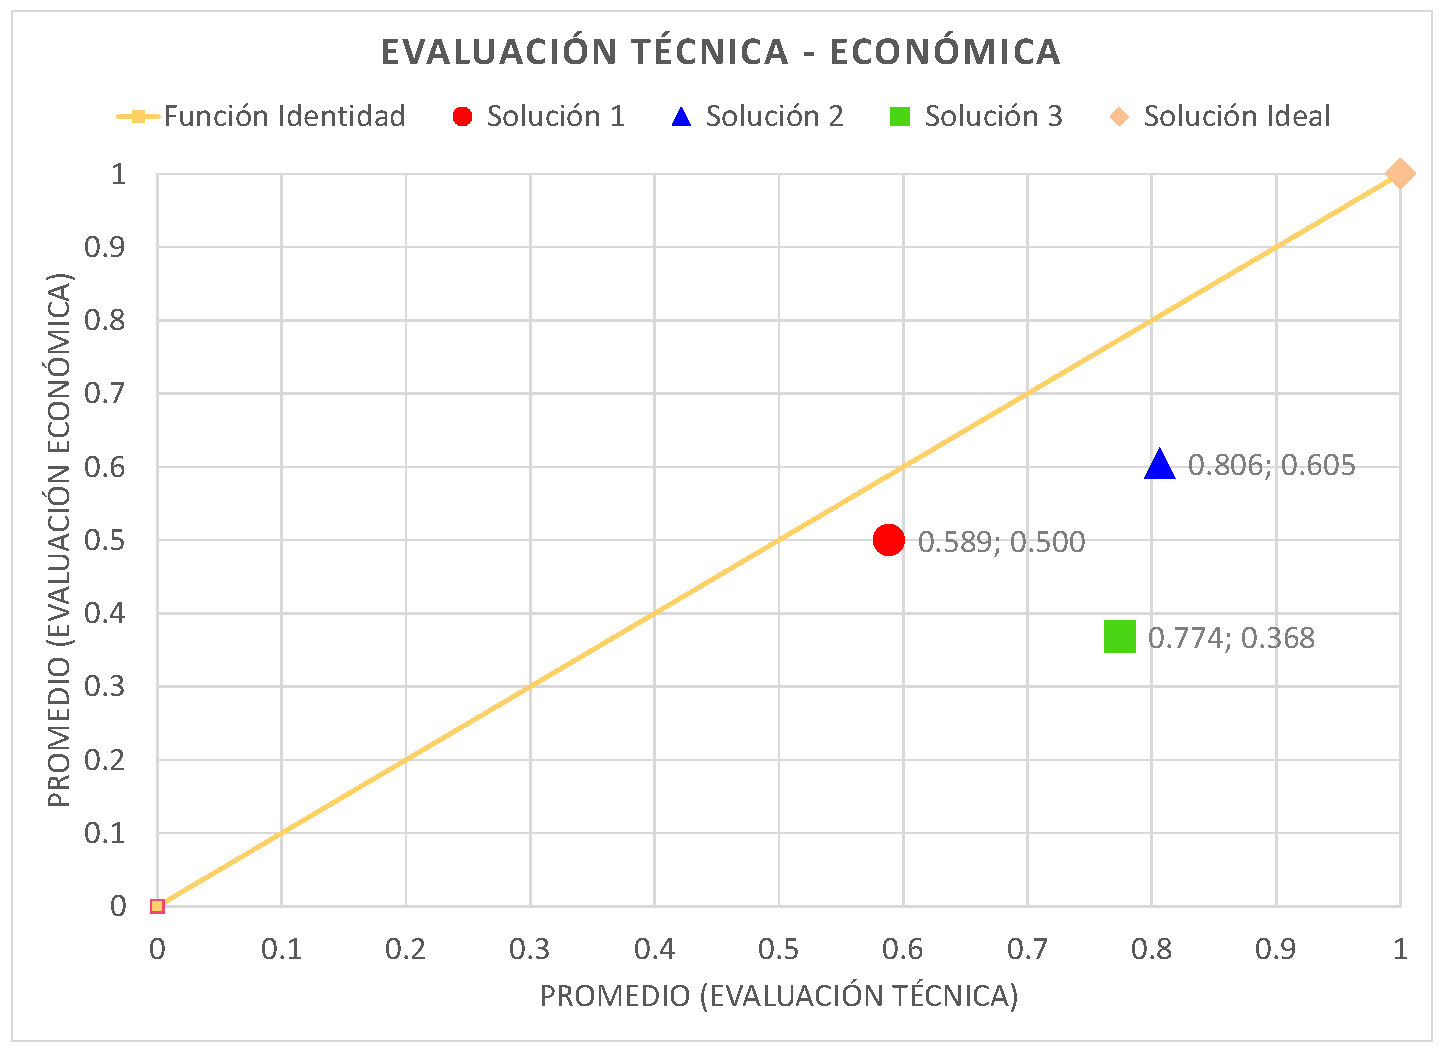
\includegraphics[width=0.8\textwidth]{img/EVALUACIONES.pdf}
	\caption[Gráfica de comparación técnico-económica de los conceptos de solución.]{Gráfica de comparación técnico-económica de los conceptos de solución. Fuente: Elaboración propia.}
	\label{fig:comp_tecnico_economica}
\end{figure}

\section{Diagrama de funcionamiento del concepto de solución óptimo}

\begin{figure}[H]
	\centering
	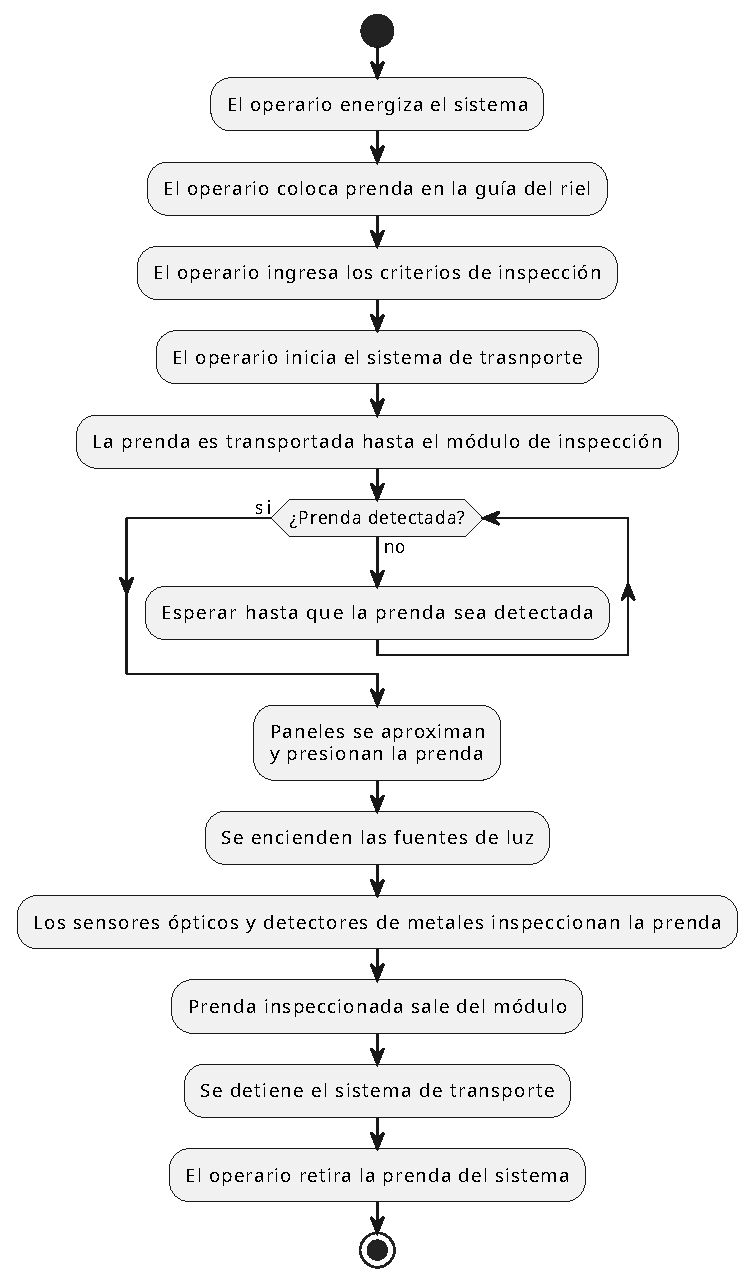
\includegraphics[width=0.8\textwidth]{img/diagrama_flujo.pdf}
	\caption[Diagrama de funcionamiento del sistema.]{Diagrama de funcionamiento del sistema. Fuente: Elaboración propia.}
	\label{fig:diagrama_flujo}
\end{figure}


%%%%% PLANEACIÓN TFC2

%\chapter*{\MakeUppercase{Planeación y Metodología para TFC2}}
\thispagestyle{mainmatterstyle} % Cambia el estilo para que este numerado en la esquina superior derecha. Esta presente en todos los chapter
%\addcontentsline{toc}{chapter}{\MakeUppercase{Planeación y Metodología para TFC2}}

\section*{Objetivos para de TFC2}
Se establece un objetivo general para el curso TFC2, del cual se derivan \ref{lst:objetivos_especificos_TFC2} objetivos específicos, donde el cumplimiento de estos, a lo largo del del curso, garantizará la consecución del objetivo principal .

\subsection*{Objetivo general}

El objetivo general para el curso TFC2 es realizar el diseño ingenieril en función al diseño conceptual óptimo elegido en TFC1.

\subsection*{Objetivos específicos}

\begin{enumerate}
	\setlength\itemsep{-0.5em}
	\item Diseñar componentes mecánicos detallados que cumplan con los requisitos funcionales y de seguridad establecidos, utilizando herramientas de diseño asistido por computadora (CAD) para su modelado y simulación.
	\item Crear esquemas eléctrico y electrónicos precisos para la implementación del proyecto, incluyendo la selección de componentes y la configuración de circuitos, garantizando la compatibilidad y funcionalidad de los sistemas.
	\item Diseñar e simular sistemas de control para la operación y desempeño del proyecto, incluyendo la programación del hardware (SBC) y sistemas embebidos.
	\item Desarrollar software personalizado para la interfaz de usuario, control, y procesamiento de datos, asegurando su integración fluida con los componentes mecánicos y electrónicos, y su usabilidad por parte de los usuarios finales.
	\item Estimar de manera precisa los costos asociados con el desarrollo de los diseños mecánicos, eléctricos/electrónicos, de sistemas de control y de software, incluyendo costos de materiales, manufactura, y operación.
	\label{lst:objetivos_especificos_TFC2}
\end{enumerate}

\section*{Metodología para alcanzar los objetivos planteados para TFC2}

Para alcanzar los objetivos específicos del curso TFC2, se propone el avance en el desarrollo del concepto de solución óptima seleccionado durante el curso TFC1. Este proceso comenzará con el diseño del sistema mecánico en la sección \ref{me_design}, donde se definirán las especificaciones dimensionales de acuerdo a los requisitos del sistema y se realizará una selección cuidadosa de materiales para cada componente. Para validar la integridad mecánica, se emplearán simulaciones de Elementos Finitos (FEA) para confirmar la rigidez y resistencia del sistema, así como simulaciones de Sistemas de Múltiples Cuerpos (MBS) para asegurar su adecuada posición espacial.

A continuación, en la sección \ref{ee_design}, se procederá con el diseño del sistema eléctrico/electrónico, que incluirá el desarrollo de esquemáticos electrónicos y un tablero eléctrico para garantizar un suministro de energía seguro al sistema. Se seleccionarán y programarán los componentes hardware necesarios.

En la sección \ref{cont_design}, se diseñará y ajustará el algoritmo de control de acuerdo con los requisitos de tiempo de funcionamiento del sistema. En la sección \ref{soft_design} se dedicará al desarrollo de una interfaz de usuario que integre Redes Neuronales Artificiales (RNA) para el procesamiento de imágenes requerido por el sistema.

Finalmente, en la sección \ref{cost_analysis}, se llevará a cabo una estimación de los costos asociados mediante el análisis de precios de componentes, costos de manufactura y operación. El proyecto concluirá con ciclos de pruebas y ajustes para asegurar el cumplimiento de los objetivos establecidos.

Para todos los diseños, se elaborarán planos detallados que incluyan dimensiones y tolerancias necesarias para la fabricación. En el caso de los diseños eléctricos/electrónicos, se especificará la lista de componentes de cada subcircuito del sistema.

%\section*{Cronograma de trabajo para TFC2}

En la Tabla \ref{tab:gantt_TFC2} se muestra el cronograma de actividades que se va a seguir para el desarrollo del trabajo de investigación del curso. La primera columna muestra el nombre de los capítulos del trabajo, mientras que la segunda columna contiene los subtítulos en los que se divide cada capítulo. Por otro lado, en color verde (\sqbox{GreenYellow}) se muestran las semanas en las que se va a redactar la sección correspondiente a cada fila. Por último, en color cian (\sqbox{cyan}) se indica la semana 9 correspondiente a la semana de exámenes parciales y en color amarillo (\sqbox{yellow}) esta indicada la semana de presentación final. 


% \usepackage{color}
% \usepackage{tabularray}
\definecolor{Sunglow}{rgb}{1,0.819,0.16}
\begin{longtblr}[caption = {Diagrama de Gantt de actividades para el curso TFC2 durante el semestre 2024-1.},label = {tab:gantt_TFC2}]{
		width = \linewidth,
		colspec = {Q[124]Q[153]Q[15]Q[15]Q[15]Q[15]Q[15]Q[15]Q[15]Q[15]Q[15]Q[19]Q[17]Q[19]Q[19]Q[19]Q[19]},
		row{1} = {c},
		row{2} = {c},
		row{3} = {c},
		row{4} = {c},
		row{5} = {Sunglow,c},
		row{6} = {c},
		column{11} = {cyan},
		column{17} = {yellow},
		cell{1}{1} = {c=17}{0.524\linewidth},
		cell{2}{2} = {c=16}{0.4\linewidth},
		cell{3}{2} = {c=16}{0.4\linewidth},
		cell{4}{2} = {c=16}{0.4\linewidth},
		cell{5}{1} = {c=2,r=2}{0.277\linewidth},
		cell{5}{3} = {c=15}{0.246\linewidth},
		cell{7}{1} = {r=2}{},
		cell{7}{3} = {green},
		cell{7}{4} = {green},
		cell{7}{5} = {green},
		cell{7}{6} = {green},
		cell{8}{3} = {green},
		cell{8}{4} = {green},
		cell{8}{5} = {green},
		cell{8}{6} = {green},
		cell{9}{1} = {r=5}{},
		cell{9}{7} = {green},
		cell{9}{8} = {green},
		cell{10}{8} = {green},
		cell{11}{9} = {green},
		cell{12}{10} = {green},
		cell{13}{15} = {green},
		cell{13}{16} = {green},
		cell{14}{1} = {r=3}{},
		cell{14}{14} = {green},
		cell{15}{14} = {green},
		cell{16}{14} = {green},
		cell{17}{15} = {green},
		cell{18}{1} = {r=3}{},
		cell{18}{13} = {green},
		cell{19}{13} = {green},
		cell{19}{14} = {green},
		cell{20}{14} = {green},
		cell{21}{1} = {r=3}{},
		cell{21}{15} = {green},
		cell{22}{15} = {green},
		cell{23}{15} = {green},
		vlines,
		hline{1-5,7,9,14,17-18,21,24} = {-}{},
		hline{8,10-13,15-16,19-20,22-23} = {2-17}{},
	}
	\documenttitle                             &                                                              &                             &   &   &   &   &   &   &   &   &    &    &    &    &    &    \\
	Elaborado por:                             & Alibert Luna Palomino                                        &                             &   &   &   &   &   &   &   &   &    &    &    &    &    &    \\
	Profesores del Curso:                      & Pedro Alonso Flores Alvarez, Jhon Manuel Portella            &                             &   &   &   &   &   &   &   &   &    &    &    &    &    &    \\
	Curso                                      & 1MTR02 - TRABAJO DE FIN DE CARRERA 2                         &                             &   &   &   &   &   &   &   &   &    &    &    &    &    &    \\
	Actividades                                &                                                              & Semanas del semestre 2024-1 &   &   &   &   &   &   &   &   &    &    &    &    &    &    \\
	&                                                              & 1                           & 2 & 3 & 4 & 5 & 6 & 7 & 8 & 9 & 10 & 11 & 12 & 13 & 14 & 15 \\
	& Verificación y corrección del documento final de TFC1        &                             &   &   &   &   &   &   &   &   &    &    &    &    &    &    \\
	& Cronograma de trabajo                                        &                             &   &   &   &   &   &   &   &   &    &    &    &    &    &    \\
	Capítulo 3:~Diseño Mecánico                & Subsistema de inspección                                     &                             &   &   &   &   &   &   &   &   &    &    &    &    &    &    \\
	& Subsistema de transporte                                     &                             &   &   &   &   &   &   &   &   &    &    &    &    &    &    \\
	& Selección de materiales                                      &                             &   &   &   &   &   &   &   &   &    &    &    &    &    &    \\
	& Subsistema del actuador lineal motorizado                    &                             &   &   &   &   &   &   &   &   &    &    &    &    &    &    \\
	& Planos                                                       &                             &   &   &   &   &   &   &   &   &    &    &    &    &    &    \\
	Capítulo 4: Diseño Eléctrico y Electrónico & Diagrama de bloques                                          &                             &   &   &   &   &   &   &   &   &    &    &    &    &    &    \\
	& Cálculos de potencia                                         &                             &   &   &   &   &   &   &   &   &    &    &    &    &    &    \\
	& Selección de componentes                                     &                             &   &   &   &   &   &   &   &   &    &    &    &    &    &    \\
	Capítulo 5:~Diseño de Control              & Diagrama de flujo y operaciones del sistema                  &                             &   &   &   &   &   &   &   &   &    &    &    &    &    &    \\
	Capítulo 6: Diseño de Software             & Desarrollo de la GUI                                         &                             &   &   &   &   &   &   &   &   &    &    &    &    &    &    \\
	& Algoritmo de visión artificial para la detección de defectos &                             &   &   &   &   &   &   &   &   &    &    &    &    &    &    \\
	& Algoritmo de visión artificial para la detección de medidas  &                             &   &   &   &   &   &   &   &   &    &    &    &    &    &    \\
	Capítulo 7: Costos                         & Costos de componentes comerciales                            &                             &   &   &   &   &   &   &   &   &    &    &    &    &    &    \\
	& Costos de diseño y fabricación                               &                             &   &   &   &   &   &   &   &   &    &    &    &    &    &    \\
	& Costos totales de fabricación                                &                             &   &   &   &   &   &   &   &   &    &    &    &    &    &    
\end{longtblr}

%\begin{longtblr}[
%	caption = {Diagrama de Gantt de actividades para el curso TFC2 durante el semestre 2024-1.},
%	label = {tab:gantt_TFC2}
%	]{
%		width = \linewidth,
%		colspec = {Q[160]Q[190]Q[11]Q[11]Q[11]Q[11]Q[11]Q[11]Q[11]Q[11]Q[11]Q[15]Q[15]Q[15]Q[15]Q[15]Q[15]},
%		row{1} = {c},
%		row{2} = {c},
%		row{3} = {c},
%		row{4} = {c},
%		row{5} = {GoldenTainoi,c},
%		row{6} = {c},
%		column{11} = {cyan},
%		column{17} = {yellow},
%		cell{1}{1} = {c=17}{0.7\linewidth},
%		cell{2}{2} = {c=16}{0.5\linewidth},
%		cell{3}{2} = {c=16}{0.5\linewidth},
%		cell{4}{2} = {c=16}{0.5\linewidth},
%		cell{5}{1} = {c=2,r=2}{0.3\linewidth},
%		cell{5}{3} = {c=15}{0.3\linewidth},
%		cell{7}{1} = {r=2}{},
%		cell{7}{3} = {GreenYellow},
%		cell{7}{4} = {GreenYellow},
%		cell{7}{5} = {GreenYellow},
%		cell{7}{6} = {GreenYellow},
%		cell{8}{3} = {GreenYellow},
%		cell{8}{4} = {GreenYellow},
%		cell{8}{5} = {GreenYellow},
%		cell{8}{6} = {GreenYellow},
%		cell{9}{1} = {r=5}{},
%		cell{9}{6} = {GreenYellow},
%		cell{9}{7} = {GreenYellow},
%		cell{10}{7} = {GreenYellow},
%		cell{11}{7} = {GreenYellow},
%		cell{12}{7} = {GreenYellow},
%		cell{13}{8} = {GreenYellow},
%		cell{14}{1} = {r=5}{},
%		cell{14}{8} = {GreenYellow},
%		cell{15}{8} = {GreenYellow},
%		cell{16}{9} = {GreenYellow},
%		cell{17}{9} = {GreenYellow},
%		cell{18}{10} = {GreenYellow},
%		cell{19}{1} = {r=2}{},
%		cell{19}{12} = {GreenYellow},
%		cell{20}{12} = {GreenYellow},
%		cell{21}{1} = {r=2}{},
%		cell{21}{13} = {GreenYellow},
%		cell{21}{14} = {GreenYellow},
%		cell{22}{13} = {GreenYellow},
%		cell{22}{14} = {GreenYellow},
%		cell{23}{1} = {r=3}{},
%		cell{23}{15} = {GreenYellow},
%		cell{23}{16} = {GreenYellow},
%		cell{24}{15} = {GreenYellow},
%		cell{24}{16} = {GreenYellow},
%		cell{25}{15} = {GreenYellow},
%		cell{25}{16} = {GreenYellow},
%		vlines,
%		hline{1-5,7,9,14,19,21,23,26} = {-}{},
%		hline{6} = {3-17}{},
%		hline{8,10-13,15-18,20,22,24-25} = {2-17}{},
%	}
%	\documenttitle & & & & & & & & & & & & & & & & \\
%	Elaborado por: & Alibert Luna Palomino & & & & & & & & & & & & & & & \\
%	Profesores del Curso: & Pedro Alonso Flores Alvarez, Jhon Manuel Portella & & & & & & & & & & & & & & & \\
%	Curso & 1MTR02 - TRABAJO DE FIN DE CARRERA 2 & & & & & & & & & & & & & & & \\
%	Actividades & & Semanas del semestre 2024-1 & & & & & & & & & & & & & & \\
%	& & 1 & 2 & 3 & 4 & 5 & 6 & 7 & 8 & 9 & 10 & 11 & 12 & 13 & 14 & 15 \\
%	& Verificación y corrección del documento final de TFC1 & & & & & & & & & & & & & & & \\
%	& Cronograma de trabajo & & & & & & & & & & & & & & & \\
%	Capítulo 3:~Diseño Mecánico & Análisis de mecanismos para transmisión de movimiento & & & & & & & & & & & & & & & \\
%	& Análisis de mecanismos para transmisión de potencia & & & & & & & & & & & & & & & \\
%	& Selección de materiales & & & & & & & & & & & & & & & \\
%	& Modelo 3D del ensamble final & & & & & & & & & & & & & & & \\
%	& Planos & & & & & & & & & & & & & & & \\
%	Capítulo 4: Diseño Eléctrico y Electrónico & Selección de componentes & & & & & & & & & & & & & & & \\
%	& Cálculos de potencia & & & & & & & & & & & & & & & \\
%	& Programación de hardware & & & & & & & & & & & & & & & \\
%	& Diagrama de conexiones & & & & & & & & & & & & & & & \\
%	& Planos & & & & & & & & & & & & & & & \\
%	Capítulo 5:~Diseño de Control & Diagrama de flujo y operaciones del sistema & & & & & & & & & & & & & & & \\
%	& Simulación de código & & & & & & & & & & & & & & & \\
%	Capítulo 6: Diseño de Software & Desarrollo de interfaz de usuario & & & & & & & & & & & & & & & \\
%	& Implementación de la RNA & & & & & & & & & & & & & & & \\
%	Capítulo 7: Costos & Costos de componentes comerciales & & & & & & & & & & & & & & & \\
%	& Costos de materia prima y fabricación & & & & & & & & & & & & & & & \\
%	& Costos totales de fabricación & & & & & & & & & & & & & & & 
%\end{longtblr}

%%%%% CAPÍTULO 4 - DISEÑO DE INGENIERÍA

%\input{chapters/preliminary_design_aspects}
%\input{chapters/mech_design}
%\input{chapters/elel_design}
%\input{chapters/soft_design}
%\input{chapters/cont_design}

%%%%% CAPÍTULO 5 - ANÁLISIS DE COSTOS

%\input{chapters/cost_analysis}

%%%%% CONCLUSIONES

%\input{chapters/conclusions}

\backmatter

%==========================================================================

\onehalfspacing % Interlineado doble para la bibliografía

%%%%% BIBLIOGRAFÍA

\cleardoublepage
\pagestyle{plain} % o el estilo que estés usando
\bibliographystyle{IEEEtran}
\bibliography{library}

%==========================================================================

\doublespacing % Interlineado doble para la bibliografía

%%%%%% ANEXOS

\appendix % Los capítulos (clase book) que siguen son tratados como apéndices.
\renewcommand\thefigure{\thesection.\arabic{figure}}
\renewcommand\thetable{\thesection.\arabic{table}}
\chapter*{ANEXOS}% If \appendix doesn't insert a \chapter
\thispagestyle{mainmatterstyle} % Cambia el estilo para que este numerado en la esquina superior derecha. Esta presente en todos los chapter
\addcontentsline{toc}{chapter}{ANEXOS}% Print Appendix in ToC
\setcounter{section}{0}% Reset numbering for sections
\setcounter{table}{0}
\setcounter{figure}{0}
\renewcommand{\thesection}{\Alph{section}}% Adjust section printing (from here onward)
\renewcommand{\thesubsection}{\Alph{section}.\arabic{subsection}}% Adjust section printing (from here onward)
\addtocontents{toc}{\protect\setcounter{tocdepth}{1}}% This turns off subsections in toc


%\section{Lista de exigencias} \label{app:list_of_demands}
%\begin{xltabular}{\textwidth}[H]{|C{1.7cm}|C{1.8cm}|X|C{2.2cm}|}
	\caption[Lista de Requerimientos.]{Lista de Exigencias. Fuente: Elaboración propia.}\label{tab:lista_exigencias}\\
	\hline
	\multicolumn{4}{|c|}{\textbf{LISTA DE EXIGENCIAS}} \bigstrut\\
	\hline
	\multicolumn{2}{|c|}{\textbf{PROYECTO}} & \centering\documenttitle & Fecha: 18/04/24 \bigstrut\\
	\hline
	\multicolumn{2}{|c|}{\textbf{CLIENTE}} & \centering\universityname & Elaborado por: \documentauthorabbreviation \bigstrut\\
	\hline
	\multicolumn{2}{|c|}{\textbf{FUNCIÓN PRINCIPAL}} & \multicolumn{2}{p{9.5cm}|}{Realizar la inspección óptica de prendas de vestir para garantizar su calidad.} \bigstrut\\
	\hline
	\textbf{Fecha} & \textbf{\makecell{Deseo o\\Exigencia}} & \centering\textbf{Descripción} & \textbf{Responsable} \bigstrut\\
	\hline
	\endfirsthead
	\caption* {Tabla \ref{tab:lista_exigencias}: Lista de Requerimientos (Continuación).}\\
	\hline
	\textbf{Fecha} & \textbf{Deseo o Exigencia} & \centering\textbf{Descripción} & \textbf{Responsable} \bigstrut\\
	\hline
	\endhead
	\multicolumn{4}{|c|}{\textbf{FUNCIONES}} \bigstrut\\
	\hline
	18/04/24 & E & La prenda ingresará de manera estirada y sin arrugas. & \documentauthorabbreviation \bigstrut\\
	\hline
	18/04/24 & E & Se debe detectar las manchas, hilos salidos y agujeros presentes en las prendas. & \documentauthorabbreviation \bigstrut\\
	\hline
	18/04/24 & E & Se debe detectar metales presentes que se hayan dejado en las prendas como agujas o alfileres. & \documentauthorabbreviation \bigstrut\\
	\hline
	\multicolumn{4}{|c|}{\textbf{OPERACIÓN}} \bigstrut\\
	\hline
	18/04/24 & E & El sistema deberá poder controlar la calidad de como mínimo 30 prendas/hora. & \documentauthorabbreviation \bigstrut\\
	\hline
	\multicolumn{4}{|c|}{\textbf{ALIMENTACIÓN}} \bigstrut\\
	\hline
	18/04/24 & E & El suministro de energía eléctrica será de 220VAC 60Hz (Monofásica). & \documentauthorabbreviation \bigstrut\\
	\hline
	\multicolumn{4}{|c|}{\textbf{SOFTWARE}} \bigstrut\\
	\hline
	18/04/24 & D & Se debe emplear un software, algoritmo o modelo de código abierto para la inspección óptica de la prenda. & \documentauthorabbreviation \bigstrut\\
	\hline
	18/04/24 & E & El sistema debe disponer de una GUI para la interacción con los operarios. & \documentauthorabbreviation \bigstrut\\
	\hline
	18/04/24 & E & 	La lógica de programación debe garantizar que los subsistemas de la máquina no tengan tiempo fuera. & \documentauthorabbreviation \bigstrut\\
	\hline
	\multicolumn{4}{|c|}{\textbf{SEÑALES}} \bigstrut\\
	\hline
	18/04/24 & E & Entrada: Encendido, apagado, inicio de proceso, fin de proceso.\newline{}Salida: Luz piloto de alimentación, encendido y funcionamiento. & \documentauthorabbreviation \bigstrut\\
	\hline
	\multicolumn{4}{|c|}{\textbf{INTERFAZ}} \bigstrut\\
	\hline
	18/04/24 & E & Tablero de control con:\newline{}- Llave de encendido general.\newline{}- Pulsador de inicio y parada de proceso.\newline{}- Parada de emergencia manual.\newline{}- Indicadores luminosos de alimentación, funcionamiento encendido.& \documentauthorabbreviation \bigstrut\\
	\hline
	18/04/24 & E & Para el diseño de la interfaz se seguirá la Norma ISO 9241, enfocada a la usabilidad y ergonomía de software y hardware. & \documentauthorabbreviation \bigstrut\\
	\hline
	\multicolumn{4}{|c|}{\textbf{CONDICIONES DE OPERACIÓN}} \bigstrut\\
	\hline
	18/04/24 & E & Ambiente de trabajo con humedad relativa máxima de 85\%, a 100 msmn (condiciones de la costa peruana, en un laboratorio de pruebas). & \documentauthorabbreviation \bigstrut\\
	\hline
	18/04/24 & D & Ambiente de trabajo industrial, con máquinas contiguas trabajando en paralelo. & \documentauthorabbreviation \bigstrut\\
	\hline
	\multicolumn{4}{|c|}{\textbf{CONTROL}} \bigstrut\\
	\hline
	18/04/24 & E & Alimentación de ropa manual hecha por un operario. & \documentauthorabbreviation \bigstrut\\
	\hline
	18/04/24 & E & Detección de defectos (manchas, hilos salidos, agujeros) automática . & \documentauthorabbreviation \bigstrut\\
	\hline
	18/04/24 & E & Detección de medidas automática de acuerdo a la ficha técnica de la prenda. & \documentauthorabbreviation \bigstrut\\
	\hline
	18/04/24 & D & Regulación de velocidad de procesamiento de prendas. & \documentauthorabbreviation \bigstrut\\
	\hline
	18/04/24 & E & Sensores grado mínimo IP 63 (resistencia al polvo y humedad condensada). & \documentauthorabbreviation \bigstrut\\
	\hline
	18/04/24 & E & Parada de emergencia automática en caso de atasco o sobrecarga. & \documentauthorabbreviation \bigstrut\\
	\hline
	\multicolumn{4}{|c|}{\textbf{SEGURIDAD}} \bigstrut\\
	\hline
	18/04/24 & E & El tablero de control debe contar con protección contra polvo y liquido grado IP64. & \documentauthorabbreviation \bigstrut\\
	\hline
	18/04/24 & E & Los circuitos eléctricos y los procesos de transferencia de calor deben estar aislados del operario para evitar accidentes. Así mismo, la máquina no debe tener filos de corte expuesto. Estos requisitos de diseño son considerados como exigencias según la Ley Nº 29783 (Ley de Seguridad y Salud en el Trabajo) y la norma OHSAS 18001.  & \documentauthorabbreviation \bigstrut\\
	\hline
	\multicolumn{4}{|c|}{\textbf{CONTROL DE CALIDAD}} \bigstrut\\
	\hline
	18/04/24 & E & La detección de defectos debe tener una efectividad del 90\%. & \documentauthorabbreviation \bigstrut\\
	\hline
	18/04/24 & E & La detección de las medidas de la prenda debe tener una precisión del 90\%. & \documentauthorabbreviation \bigstrut\\
	\hline
	\multicolumn{4}{|c|}{\textbf{MONTAJE}} \bigstrut\\
	\hline
	18/04/24 & D & El sistema presenta la posibilidad de acoplar varias lineas en paralelo para incrementar la productividad. & \documentauthorabbreviation \bigstrut\\
	\hline
	18/04/24 & E & El diseño de la máquina debe ser compacto y debe permitir desmontar los componentes que requieran mantenimiento. Además, se debe considerar una conexión estándar de energía eléctrica. & \documentauthorabbreviation \bigstrut\\
	\hline
	\multicolumn{4}{|c|}{\textbf{MATERIAL}} \bigstrut\\
	\hline
	18/04/24 & E & Materiales que eviten la acumulación de manchas y polvo. & \documentauthorabbreviation \bigstrut\\
	\hline
	\multicolumn{4}{|c|}{\textbf{FABRICACIÓN}} \bigstrut\\
	\hline
	18/04/24 & E & El diseño debe contar con componentes estandarizados que estén disponibles en el mercado local. & \documentauthorabbreviation \bigstrut\\
	\hline
	18/04/24 & D & Los elementos diseñados deben evitar el mantenimiento difícil. & \documentauthorabbreviation \bigstrut\\
	\hline
	\multicolumn{4}{|c|}{\textbf{MANTENIMIENTO}} \bigstrut\\
	\hline
	18/04/24 & E & Los elementos motrices serán accesibles y las superficies fáciles de limpiar. Los componentes electrónicos no deben estar expuestas al polvo. & \documentauthorabbreviation \bigstrut\\
	\hline
	\multicolumn{4}{|c|}{\textbf{DIMENSIONES}} \bigstrut\\
	\hline
	18/04/24 & E & El sistema no deberá ocupar un volumen mayor a 4m x 3m x 3m para poder ser construido en un laboratorio. & \documentauthorabbreviation \bigstrut\\
	\hline
	18/04/24 & E & Las dimensiones y la disposición del sistema deben estar diseñadas de manera que garanticen una operación cómoda y segura para el operario. & \documentauthorabbreviation \bigstrut\\
	\hline
	\multicolumn{4}{|c|}{\textbf{COSTO}} \bigstrut\\
	\hline
	18/04/24 & D & Fabricación: 80000 PEN. & \documentauthorabbreviation \bigstrut\\
	\hline
\end{xltabular}

%
%\setcounter{table}{0}
%\setcounter{figure}{0}
%
%\section{Funciones Parciales} \label{app:partial_functions}
%\begin{figure}[H]
	\centering
	\includegraphics[width=\textwidth]{ESTRUCTURA_DE_FUNCIONES.drawio.pdf}
	\caption[Estructura de funciones del sistema.]{Estructura de funciones del sistema. Fuente: Elaboración propia.}
	\label{fig:ESTRUCTURA_DE_FUNCIONES}
\end{figure}

\subsubsection{Dominio Mecánico}

El dominio mecánico abarca todas las operaciones físicas y movimientos asociados con el manejo de prendas de vestir, como se muestra en la Figura \ref{fig:EF_DM}. Incluye la recepción de las prendas, su transporte a través de diferentes estaciones de procesamiento como módulos de detección de defectos y el módulo de detección de metales. Una vez terminada la inspección de la prenda, esta es transportada a su disposición final.

\begin{figure}[H]
	\centering
	\includegraphics[width=\textwidth]{EF_DM.pdf}
	\caption[Estructura de funciones del dominio mecánico.]{Estructura de funciones del dominio mecánico. Fuente: Elaboración propia.}
	\label{fig:EF_DM}
\end{figure}

\subsubsection{Dominio Informático}

El dominio informático se centra en el procesamiento de la información obtenida de las prendas , como se muestra en la Figura \ref{fig:EF_DIn}. Este dominio comprende la adquisición y preprocesamiento de imágenes de las prendas, extracción de características relevantes, detección de defectos, y comparación de estos datos con criterios de selección predefinidos para determinar la calidad de las prendas. Este dominio es crucial para interpretar los datos capturados y tomar decisiones basadas en la información procesada.

\begin{figure}[H]
	\centering
	\includegraphics[width=\textwidth]{EF_DIn.pdf}
	\caption[Estructura de funciones del dominio informático.]{Estructura de funciones del dominio informático. Fuente: Elaboración propia.}
	\label{fig:EF_DIn}
\end{figure}

\subsubsection{Dominio de Control}

El dominio de control, mostrado en la Figura \ref{fig:EF_DC}, incluye la lógica de control y los mecanismos de decisión que guían las operaciones del sistema. Esto implica generar señales de encendido/apagado basadas en la información procesada, manejar interfaces de entrada/salida, y activar mecanismos de parada de emergencia. Este dominio es esencial para coordinar las actividades de los otros dominios y asegurar que el sistema responda adecuadamente a las condiciones de operación y a los requisitos de procesamiento.

\begin{figure}[H]
	\centering
	\includegraphics[width=0.6\textwidth]{EF_DC.pdf}
	\caption[Estructura de funciones del dominio de control.]{Estructura de funciones del dominio de control. Fuente: Elaboración propia.}
	\label{fig:EF_DC}
\end{figure}

\subsubsection{Dominio Eléctrico/Electrónico}

El dominio mencionado se ocupa del suministro y control eléctrico de todos los componentes del sistema, como se ilustra en la Figura \ref{fig:EF_DEE}. Su función principal es proporcionar la energía necesaria para el funcionamiento de todos los componentes electrónicos del sistema, desde la activación de los sensores hasta la alimentación de los sistemas de procesamiento de información, actuadores y control. También gestiona la iluminación necesaria para la adquisición de imágenes y la señalización a través de indicadores ON/OFF.

\begin{figure}[H]
	\centering
	\includegraphics[width=0.6\textwidth]{EF_DEE.pdf}
	\caption[Estructura de funciones del dominio eléctrico/electrónico.]{Estructura de funciones del dominio eléctrico/electrónico. Fuente: Elaboración propia.}
	\label{fig:EF_DEE}
\end{figure}

\subsubsection{Dominio de Sensores}

Este dominio comprende la detección y recopilación de datos a través de sensores diseñados para identificar características específicas de las prendas. Esto se muestra en la Figura \ref{fig:EF_DS}. Se identifica la presencia de metales o la preparación para la captura de imágenes.

\begin{figure}[H]
	\centering
	\includegraphics[width=0.55\textwidth]{EF_DS.pdf}
	\caption[Estructura de funciones del dominio de sensores.]{Estructura de funciones del dominio de sensores. Fuente: Elaboración propia.}
	\label{fig:EF_DS}
\end{figure}

\subsubsection{Dominio de Interfaz}

El dominio de la interfaz está dedicado a facilitar la interacción con los usuarios finales del sistema. Como se ilustra en la Figura \ref{fig:EF_DI_1}, esta interacción implica el uso de la energía mecánica ejercida por el operario para generar las señales de control necesarias, que incluyen las acciones de encendido, apagado y parada de emergencia. Por otra parte, la Figura \ref{fig:EF_DI_2} exhibe los resultados derivados de todos los procesos ejecutados por el sistema. Estos resultados se presentan a través de una interfaz diseñada para mostrar la información de manera ordenada y concisa.

\begin{figure}[H]
	\centering
	\includegraphics[width=0.7\textwidth]{EF_DI_1.pdf}
	\caption[Estructura de funciones del dominio de interfaz.]{Estructura de funciones del dominio de interfaz. Fuente: Elaboración propia.}
	\label{fig:EF_DI_1}
\end{figure}

\begin{figure}[H]
	\centering
	\includegraphics[width=0.7\textwidth]{EF_DI_1.pdf}
	\caption[Estructura de funciones del dominio de interfaz.]{Estructura de funciones del dominio de interfaz. Fuente: Elaboración propia.}
	\label{fig:EF_DI_2}
\end{figure}
%
%\setcounter{table}{0}
%\setcounter{figure}{0}
%
%\section{Matriz morfológica} \label{app:morphological_matrix_tables}
%\begin{table}[H]
	\centering
	\captionsetup{justification=centering}
	\caption[Leyenda de colores para los conceptos de solución en las matriz morfológica.]{Leyenda de colores para los conceptos de solución en las matriz morfológica.\\Fuente: Elaboración propia.}
	\begin{tabular}{|c|c|c|}
		\hline
		\textbf{Soluciones} & \textbf{Tipo de Solución} & \textbf{Color} \bigstrut\\
		\hline
		Solución 1 & Accesible & \cellcolor[rgb]{1,0,0} \bigstrut\\
		\hline
		Solución 2 & Precisa & \cellcolor[rgb]{0,0,1} \bigstrut\\
		\hline
		Solución 3 & Robusta & \cellcolor[rgb]{.298, .835, .078} \bigstrut\\
		\hline
	\end{tabular}%
	\label{tab:leyenda_colores_soluciones}%
\end{table}

\subsection{Dominio de Interfaz}

\begin{xltabular}{\textwidth}{|M{4cm}|Y|Y|Y|}
	% CONFIGURACIÓN Y CABECERA DE LA TABLA
	\caption{Matriz morfológica del dominio de interfaz.}\label{tab:MM_DI}\\
	\hline
	\multirow{2}{*}{{\textbf{\minitab[c]{FUNCIONES\\PARCIALES}}}} & \multicolumn{3}{c|}{\textbf{DOMINIO INTERFAZ}}\\
	\cline{2-4} & \textbf{OPCIÓN 1} & \textbf{OPCIÓN 2} & \textbf{OPCIÓN 3}\\
	\hline
	\endfirsthead
	\caption*{Tabla \ref{tab:MM_DI}: Matriz morfológica del dominio de interfaz (Continuación).}\\
	\hline
	\multirow{2}{*}{\textbf{\minitab[c]{FUNCIONES\\PARCIALES}}} & \multicolumn{3}{c|}{\textbf{DOMINIO INTERFAZ}}\\
	\cline{2-4} & \textbf{OPCIÓN 1} & \textbf{OPCIÓN 2} & \textbf{OPCIÓN 3}\\
	\hline
	\endhead
	% INICIO DE LA TABLA
	\multirow[b]{2}{*}{\minitab[c]{GENERAR SEÑAL\\ON Y GENERAR\\SEÑAL OFF}} & \IMM{0.06}{botonera1.jpg}{2pt} & \IMM{0.1}{boton_enc_apa_GUI.jpg}{0.6pt} & \IMM{0.11}{Switch_tipo_perilla.jpeg}{2pt} \\
	\cline{2-4} & \minitab[c]{Caja con\\pulsador\\Start-Stop.\\ \OpV} & \minitab[c]{Botones\\ON/OFF\\en GUI.\\ \OpR} & \minitab[c]{Interruptor\\tipo perilla.\\\OpA} \\
	\hline
	\multirow[t]{2}{*}{\minitab[c]{ENCENDER\\INDICADOR DE\\ON, DE OFF Y DE\\ALIMENTACIÓN}} & \IMM{0.13}{img/pilotos_led.jpg}{0.5em} & \IMM{0.14}{img/pantalla_LCD.jpg}{0.3em} & \IMM{0.15}{img/GUI.jpg}{0.1em} \\
	\cline{2-4} & \minitab[c]{Pilotos led.\\\OpV} & \minitab[c]{Pantalla LCD.\\\OpR} & \minitab[c]{GUI.\\\OpA} \\
	\hline
	\multirow{2}{*}{\minitab[c]{RECIBIR\\CRITERIOS DE\\SELECCIÓN}} & \IMM{0.13}{img/hmi_industrial.png}{0.2em} & \IMM{0.15}{img/Pantalla_Perilla.jpg}{0.24em} & \IMM{0.15}{img/GUI.jpg}{0.1em} \\
	\cline{2-4} & \minitab[c]{HMI\\Industrial.\\\OpA} & \minitab[c]{Pantalla LCD\\con perilla\\de control.\\\OpR} & \minitab[c]{GUI.\\\OpV} \\
	\hline
	\multirow{2}{*}{\minitab[c]{CONECTAR Y\\CORTAR\\ALIMENTACIÓN\\ELÉCTRICA}} & \IMM{0.12}{img/termomagnético_diferencial.jpg}{0.7em} & \IMM{0.11}{img/Conmutador_industrial.jpeg}{0.2em} & \IMM{0.11}{img/cable_interruptor.jpg}{0.1em} \\
	\cline{2-4} & \minitab[c]{Diferencial con\\Termomagnético.\\\OpV} & \minitab[c]{Conmutador\\Industrial.\\\OpA} & \minitab[c]{Cable,\\enchufe e\\interruptor.\\\OpR} \\
	\hline
	\multirow{2}{*}{\minitab[c]{MOSTRAR\\INFORMACIÓN\\GRÁFICAMENTE}} & \IMM{0.12}{img/hmi_industrial.png}{0.3em} & \IMM{0.15}{img/GUI.jpg}{0.1em} & \\
	\cline{2-4} & \minitab[c]{HMI\\Industrial.\\\OpA} & \minitab[c]{GUI.\\\OpR \OpV} & \\
	\hline
\end{xltabular}


\subsection{Dominio Mecánico}

\begin{xltabular}{\textwidth}{|M{4cm}|Y|Y|Y|}
	\caption{Matriz morfológica del dominio mecánico.}\label{tab:MM_DM}\\
	\hline
	\multirow{2}{*}{\textbf{\minitab[c]{FUNCIONES\\PARCIALES}}} & \multicolumn{3}{c|}{\textbf{DOMINIO MECÁNICO}}\\
	\cline{2-4} & \textbf{OPCIÓN 1} & \textbf{OPCIÓN 2} & \textbf{OPCIÓN 3}\\
	\hline
	\endfirsthead
	\caption*{Tabla \ref{tab:MM_DM}: Matriz morfológica del dominio mecánico (Continuación).}\\
	\hline
	\multirow{2}{*}{\textbf{\minitab[c]{FUNCIONES\\PARCIALES}}} & \multicolumn{3}{c|}{\textbf{DOMINIO MECÁNICO}}\\
	\cline{2-4} & \textbf{OPCIÓN 1} & \textbf{OPCIÓN 2} & \textbf{OPCIÓN 3}\\
	\hline
	\endhead
	\multirow[t]{2}{*}{\minitab[c]{TRANSPORTE\\MECÁNICO DE\\LAS PRENDAS\\DE VESTIR}} & \IMM{0.14}{img/faja_transportadora_plana.jpg}{0.2em} & \IMM{0.13}{img/faja_transportadora_inclinada.jpg}{0.8em}& \IMM{0.11}{img/conveyer.jpg}{0.2em} \\
	\cline{2-4} & \minitab[c]{Faja\\transportadora\\plana.\\\OpR} & \minitab[c]{Faja\\transportadora\\inclinada.\\\OpA} & \minitab[c]{Transportador\\automático\\de ropa.\\\OpV} \\
	\hline    
	\multirow[t]{2}{*}{\minitab[c]{GENERAR EL\\MOVIMIENTO\\DEL SISTEMA\\DE TRANSPORTE}} & \IMM{0.15}{stepper_motor.jpg}{0.3em} & \IMM{0.15}{motor_sincrono.jpg}{0.1em}& \IMM{0.14}{motor_asincrono.jpg}{0.2em} \\
	\cline{2-4} & \minitab[c]{Motor a\\pasos.\\\OpV} & \minitab[c]{Motor\\síncrono.\\\OpA} & \minitab[c]{Motor de\\inducción.\\\OpR} \\
	\hline
\end{xltabular}

\subsection{Dominio Informático}

\begin{xltabular}{\textwidth}{|M{4cm}|Y|Y|Y|}
	\caption{Matriz morfológica del dominio informático.}\label{tab:MM_DIn}\\
	\hline
	\multirow{2}{*}{\textbf{\minitab[c]{FUNCIONES\\PARCIALES}}} & \multicolumn{3}{c|}{\textbf{DOMINIO INFORMÁTICO}} \bigstrut\\
	\cline{2-4} & \textbf{OPCIÓN 1} & \textbf{OPCIÓN 2} & \textbf{OPCIÓN 3} \bigstrut\\
	\hline
	\endfirsthead
	\caption*{Tabla \ref{tab:MM_DIn}: Matriz morfológica del dominio informático (Continuación).}\\
	\hline
	\multirow{2}{*}{\textbf{\minitab[c]{FUNCIONES\\PARCIALES}}} & \multicolumn{3}{c|}{\textbf{DOMINIO INFORMÁTICO}} \bigstrut\\
	\cline{2-4} & \textbf{OPCIÓN 1} & \textbf{OPCIÓN 2} & \textbf{OPCIÓN 3} \bigstrut\\
	\hline
	\endhead
	\multirow[t]{2}{*}{\minitab[c]{IDENTIFICAR E\\INTERPRETAR LAS\\SEÑALES}} & \IMM{0.13}{img/computadora_industrial.png}{0.5em} & \IMM{0.14}{img/SBC.jpg}{0.3em} & \IMM{0.14}{img/micro.jpg}{0.3em} \bigstrut\\
	\cline{2-4} & \minitab[c]{Computadora\\Industrial.\\\OpA} & \minitab[c]{Single Board\\Computer (SBC).\\\OpV} & \minitab[c]{Micro-\\controlador.\\\OpR} \bigstrut\\
	\hline
	\multirow[t]{2}{*}{\minitab[c]{ALMACENAR\\CRITERIOS DE\\SELECCIÓN}} & \IMM{0.11}{img/memoria_sd.jpg}{0.1em} & \IMM{0.12}{img/memoria_tera.jpg}{0.1em} & \IMM{0.12}{img/memoria_ssd.jpg}{0.1em} \bigstrut\\
	\cline{2-4} & \minitab[c]{Memoria SD.\\\OpV} & \minitab[c]{Memoria\\Externa.\\\OpR} & \minitab[c]{Memoria\\Interna.\\\OpA} \bigstrut\\*
	\hline
	\pagebreak
	\multirow[t]{2}{*}{\minitab[c]{PROCESAR\\IMÁGENES}} & \IMM{0.1}{img/opencv.png}{0.5em} & \IMM{0.11}{img/matlab.png}{0.2em} & \IMM{0.12}{img/code.png}{0.2em} \bigstrut\\
	\cline{2-4} & \minitab[c]{OpenCV\\(Python).\\\OpV} & \minitab[c]{MATLAB.\\\OpA} & \minitab[c]{Programación\\Nativa.\\\OpR} \bigstrut\\
	\hline
	\multirow[t]{2}{*}{\minitab[c]{DETECTAR\\DEFECTOS Y\\MEDIDAS}} & \IMM{0.13}{img/yolov8.jpg}{0.1em} & \IMM{0.13}{img/fasterRCNN.png}{0.1em} & \IMM{0.12}{img/analisis_clasico.png}{0.2em} \bigstrut\\
	\cline{2-4} & \minitab[c]{YOLOv8.\\\OpV} & \minitab[c]{Fast R-CNN.\\\OpA} & \minitab[c]{Análisis\\Clásico.\\\OpR} \bigstrut\\
	\hline
\end{xltabular}


\subsection{Dominio de Control}

\begin{xltabular}{\textwidth}{|M{4cm}|Y|Y|Y|}
	\caption{Matriz morfológica del dominio de control.}\label{tab:MM_DC}\\
	\hline
	\multirow{2}{*}{\textbf{\minitab[c]{FUNCIONES\\PARCIALES}}} & \multicolumn{3}{c|}{\textbf{DOMINIO DE CONTROL}} \bigstrut\\
	\cline{2-4} & \textbf{OPCIÓN 1} & \textbf{OPCIÓN 2} & \textbf{OPCIÓN 3} \bigstrut\\
	\hline
	\endfirsthead
	\caption*{Tabla \ref{tab:MM_DC}: Matriz morfológica del dominio de control (Continuación).}\\
	\hline
	\multirow{2}{*}{\textbf{\minitab[c]{FUNCIONES\\PARCIALES}}} & \multicolumn{3}{c|}{\textbf{DOMINIO DE CONTROL}} \bigstrut\\
	\cline{2-4} & \textbf{OPCIÓN 1} & \textbf{OPCIÓN 2} & \textbf{OPCIÓN 3} \bigstrut\\
	\hline
	\endhead
	\multirow[t]{2}{*}{\minitab[c]{ELEMENTO DE\\CONTROL}} & \IMM{0.15}{img/ESP32.jpg}{0.08em} & \IMM{0.14}{img/raspberry.jpg}{0.1em} & \IMM{0.14}{img/plc.jpg}{0.1em} \bigstrut\\
	\cline{2-4} & \minitab[c]{Microcontrolador.\\\OpR} & \minitab[c]{Single Board\\Computer (SBC).\\\OpV} & \minitab[c]{PLC.\\\OpA} \bigstrut\\
	\hline
	\pagebreak
	\multirow[t]{2}{*}{\minitab[c]{ALGORITMO DE\\CONTROL}} & \IMM{0.16}{img/PID_DISCRETO.png}{0.1em} & \IMM{0.16}{img/onoff_control.png}{0.1em} & \IMM{0.15}{img/realimentacion_estados.png}{0.08em} \bigstrut\\
	\cline{2-4} & \minitab[c]{PID\\Discreto.\\\OpA} & \minitab[c]{Control\\ON OFF.\\\OpR} & \minitab[c]{Retroalimentación\\de Estados.\\\OpV} \bigstrut\\
	\hline
\end{xltabular}

\subsection{Dominio Eléctrico/Electrónico}

\begin{xltabular}{\textwidth}{|C{5cm}|Y|Y|Y|}
	\caption{Matriz morfológica del dominio eléctrico/electrónico.}\label{tab:MM_DEE}\\
	\hline
	\multirow{2}{*}{\textbf{\minitab[c]{FUNCIONES\\PARCIALES}}} & \multicolumn{3}{c|}{\textbf{DOMINIO ELÉCTRICO/ELECTRÓNICO}} \bigstrut\\
	\cline{2-4} & \textbf{OPCIÓN 1} & \textbf{OPCIÓN 2} & \textbf{OPCIÓN 3} \bigstrut\\
	\hline
	\endfirsthead
	\caption*{Tabla \ref{tab:MM_DEE}: Matriz morfológica del dominio eléctrico/electrónico (Continuación).}\\
	\hline
	\multirow{2}{*}{\textbf{\minitab[c]{FUNCIONES\\PARCIALES}}} & \multicolumn{3}{c|}{\textbf{DOMINIO ELÉCTRICO/ELECTRÓNICO}} \bigstrut\\
	\cline{2-4} & \textbf{OPCIÓN 1} & \textbf{OPCIÓN 2} & \textbf{OPCIÓN 3} \bigstrut\\
	\hline
	\endhead
	\multirow[t]{2}{*}{\minitab[c]{ACONDICIONAR\\ENERGÍA\\ELÉCTRICA}} & \IMM{0.13}{img/fuente_switching.jpg}{0.1em} & \IMM{0.13}{img/circuito_rectificador.jpg}{0.1em} & \IMM{0.13}{img/adaptador_AC_DC.jpg}{0.1em} \bigstrut\\
	\cline{2-4} & \minitab[c]{Fuente\\Switching.\\\OpV} & \minitab[c]{Rectificado\\AC/DC.\\\OpR} & \minitab[c]{Adaptador\\AC a DC.\\\OpA} \bigstrut\\
	\hline
	\multirow[b]{2}{*}{\minitab[c]{ACTIVAR\\SISTEMA DE\\PARADA DE\\EMERGENCIA}} & \IMM{0.12}{img/boton_parada_emergencia.jpg}{0.5em} &  &  \bigstrut\\
	\cline{2-4} & \minitab[c]{Botón de\\parada de\\emergencia.\\\OpR \OpA \OpV} &  &  \bigstrut\\
	\hline
	\pagebreak
	\multirow[b]{2}{*}{\minitab[c]{ENERGIZAR SIST. DE\\CONTROL, SENSORES,\\PROC. INFORMACIÓN\\Y MECÁNICO}} & \IMM{0.13}{img/cables_terminal_crimpado.jpg}{0.1em} & \IMM{0.13}{img/cable_motor.jpg}{0.1em} & \bigstrut\\
	\cline{2-4} & \minitab[c]{Cables con\\los terminales\\crimpados.\\\OpR \OpV} & \minitab[c]{Cables de\\motor.\\\OpA} & \bigstrut\\
	\hline
	\multirow[b]{2}{*}{\minitab[c]{ALIMENTAR\\SISTEMA DE\\PROCESAMIENTO\\DE LA\\INFORMACIÓN}} & \IMM{0.11}{img/cable_usb_micro.jpg}{0.1em} & \IMM{0.12}{img/cable_usb_usbB.jpg}{0.5em} & \\
	\cline{2-4} & \minitab[c]{Cable USB\\Tipo A a\\microUSB.\\\OpR \OpV} & \minitab[c]{Cable USB\\Tipo A a\\Tipo B.\\\OpA} & \bigstrut\\
	\hline
	\multirow[t]{2}{*}{\minitab[c]{ENCENDER LA\\ILUMINACIÓN\\ARTIFICIAL}} & \IMM{0.17}{img/panel_de_luz.jpg}{0.12em} & \IMM{0.13}{img/tira_led.png}{0.2em} & \bigstrut\\
	\cline{2-4} & \minitab[c]{Panel de luz.\\\OpA \OpV} & \minitab[c]{Tira LED.\\\OpR} & \bigstrut\\
	\hline
\end{xltabular}

\newpage

\subsection{Dominio de Sensores}

\begin{xltabular}{\textwidth}{|M{4cm}|Y|Y|Y|}
	\caption{Matriz morfológica del dominio de sensores.}\label{tab:MM_DS}\\
	\hline
	\multirow{2}{*}{\textbf{\minitab[c]{FUNCIONES\\PARCIALES}}} & \multicolumn{3}{c|}{\textbf{DOMINIO DE SENSORES}} \bigstrut\\
	\cline{2-4} & \textbf{OPCIÓN 1} & \textbf{OPCIÓN 2} & \textbf{OPCIÓN 3} \bigstrut\\
	\hline
	\endfirsthead
	\caption*{Tabla \ref{tab:MM_DS}: Matriz morfológica del dominio de sensores. (Continuación).}\\
	\hline
	\multirow{2}{*}{\textbf{\minitab[c]{FUNCIONES\\PARCIALES}}} & \multicolumn{3}{c|}{\textbf{DOMINIO DE SENSORES}} \bigstrut\\
	\cline{2-4} & \textbf{OPCIÓN 1} & \textbf{OPCIÓN 2} & \textbf{OPCIÓN 3} \bigstrut\\
	\hline
	\endhead
	\multirow[b]{2}{*}{\minitab[c]{ADQUIRIR\\IMAGEN}} & \IMM{0.13}{img/camara_USB.jpg}{0.1em} & \IMM{0.13}{img/camara_industrial.jpg}{0.1em} & \IMM{0.13}{img/camara_web.jpg}{0.1em} \bigstrut\\
	\cline{2-4} & \minitab[c]{Cámara USB.\\\OpV} & \minitab[c]{Cámara\\Industrial.\\\OpA} & \minitab[c]{Cámara Web.\\\OpR} \bigstrut\\
	\hline
	\multirow[b]{2}{*}{\minitab[c]{DETECTAR\\METALES EN\\PRENDAS}} & \IMM{0.13}{img/detector_agujas.jpg}{0.1em} & \IMM{0.13}{img/detector_metales.png}{0.1em} & \bigstrut\\
	\cline{2-4} & \minitab[c]{Detector de\\Agujas.\\\OpA \OpV} & \minitab[c]{Detector de\\Metales.\\\OpR} & \bigstrut\\
	\hline
	\multirow[b]{2}{*}{\minitab[c]{DETECTAR\\PRESENCIA DE\\LA PRENDA\\PARA CAPTURA}} & \IMM{0.13}{img/sensor_proximidad_capacitivo.jpg}{0.1em} & \IMM{0.13}{img/sensor_fotoelectrico.jpg}{0.1em} & \IMM{0.13}{img/sensor_ultrasonido.jpg}{0.1em} \bigstrut\\
	\cline{2-4} & \minitab[c]{Sensor\\Capacitivo.\\\OpV} & \minitab[c]{Sensor\\Fotoeléctrico.\\\OpA} & \minitab[c]{Sensor\\Ultrasonido.\\\OpR} \bigstrut\\
	\hline
\end{xltabular}



\end{document}